\documentclass[12pt,oneside]{article}

\usepackage[a4paper,top=25mm,bottom=25mm,left=25mm,right=25mm,headheight=15pt]{geometry}
\usepackage{newtxtext}
\usepackage{newtxmath}
\usepackage{amsmath}
\usepackage{siunitx}
\usepackage{graphicx}
\usepackage{booktabs}
\usepackage{float}
\usepackage{placeins}
\usepackage{caption}
\usepackage{subcaption}
\captionsetup{labelfont=bf}
\DeclareCaptionLabelFormat{continued}{#1~#2 (cont.)}
\captionsetup[ContinuedFloat]{labelformat=continued}
\usepackage{makecell}
\usepackage{tabularx}
\usepackage{rotating}
\usepackage{tikz}
\usetikzlibrary{arrows.meta,positioning,calc,shapes.arrows}
\usepackage{fancyhdr}
\usepackage{setspace}
\usepackage{indentfirst}
\usepackage{titlesec}
\usepackage[authoryear]{natbib}
% Number bibliography entries while retaining author-year citations in the text.
\makeatletter
\renewcommand{\NAT@biblabel}[1]{\hfill[#1]}
\renewcommand{\NAT@bibsetup}[1]{\NAT@bibsetnum{#1}}
\makeatother
\usepackage{xcolor}
\usepackage{soul}
\usepackage{lineno}
\usepackage{hyperref}
\usepackage{xr-hyper}
\externaldocument[supp-]{supplement}
\usepackage{cleveref}

\onehalfspacing
\setlength{\parindent}{1.5em}
\setlength{\parskip}{0pt}
\titleformat{\section}{\normalfont\large\bfseries}{\thesection}{1em}{}
\titleformat{\subsection}{\normalfont\normalsize\bfseries}{\thesubsection}{1em}{}
\titlespacing*{\section}{0pt}{1.25\baselineskip}{0.35\baselineskip}
\titlespacing*{\subsection}{0pt}{0.55\baselineskip}{0.25\baselineskip}
\titlespacing*{\subsubsection}{0pt}{0.45\baselineskip}{0.2\baselineskip}

\pagestyle{fancy}
\fancyhf{}
\fancyhead[R]{\thepage}
\fancyhead[L]{\textit{Tuku manuscript draft}}
\renewcommand{\headrulewidth}{0.4pt}

\bibliographystyle{plainnat}
\hypersetup{
  colorlinks=true,
  linkcolor=blue,
  citecolor=blue,
  urlcolor=blue,
  % pdftitle={Monthly estimation of depth-resolved aquifer-system compaction at Tuku},
  % pdftitle={Estimating Monthly Aquifer-System Deformation by Depth under Limited Direct Measurements},
  pdftitle={Estimating Aquifer-System Deformation across Depth Sections between Direct Measurements for Land Subsidence Monitoring},
  pdfauthor={Author names to be confirmed},
  % pdfkeywords={aquifer-system compaction, groundwater level, delayed observations, Bayesian ridge regression, Tuku},
  pdfkeywords={land subsidence, aquifer-system compaction, depth-resolved deformation, multilayer compaction monitoring wells, delayed data availability, measurement frequency, Bayesian ridge regression, uncertainty quantification},
  bookmarksnumbered=true,
  bookmarksopen=true,
  pdfstartview=FitH
}

\newcommand{\keywords}[1]{\vspace{2mm}\noindent\textbf{Keywords:} #1}
\newcommand{\placeholder}[1]{\begingroup\sethlcolor{yellow}\hl{[#1]}\endgroup}

\begin{document}

\pagenumbering{roman}
% \title{\textbf{Monthly Estimation of Depth-Resolved Aquifer-System Compaction during Delayed Monitoring Data Delivery at Tuku, Taiwan}}
% \title{\textbf{Estimating Monthly Aquifer-System Deformation by Depth under Limited Direct Measurements}}
\title{\textbf{Estimating Depth-Resolved Deformation from Hydraulic and Geodetic Observations under Constrained Multilayer Compaction Measurements for Land Subsidence Monitoring}}
\author{\placeholder{AUTHOR NAMES AND AFFILIATIONS}}
\date{Draft compiled on \today}
\maketitle

\begin{abstract}
% Land subsidence develops as groundwater withdrawal increases effective stress and compacts susceptible sediments within an aquifer system. Surface displacement measurements describe the total vertical response, but they do not show how the compaction is distributed with depth. Multilayer compaction monitoring wells provide this information directly, although their monthly observations may not be available when a current assessment is required. This study tested whether routinely available monitoring data could provide provisional estimates of monthly compaction during a six-month delay in the delivery of multilayer compaction observations at Tuku, central Taiwan. The analysis represented the monitored profile by six 50~m depth sections and related their monthly compaction to hydraulic head changes, vertical surface displacement from a continuous Global Navigation Satellite System station, and seasonal terms. Bayesian ridge regression was evaluated in temporal order. Six consecutive monthly compaction observations were withheld during each evaluation period, and the model was updated only after the withheld observations became available. The updated model achieved \placeholder{POOLED R2, RMSE, AND MAE} and \placeholder{MAIN DEPTH-DEPENDENT RESULT}. Its performance was \placeholder{COMPARISON WITH FROZEN AND PERSISTENCE BASELINES}. Error-calibrated 90\% prediction intervals attained \placeholder{EMPIRICAL COVERAGE} with a mean width of \placeholder{INTERVAL WIDTH}. These results \placeholder{CONCISE OPERATIONAL CONCLUSION SUPPORTED BY THE FINAL RUN}.
Effective management of land subsidence caused by groundwater withdrawal requires information on how aquifer-system compaction is distributed with depth. Multilayer compaction monitoring well (MLCW) measurements provide this information directly, but the measurements must be processed and checked before finalized records are released, which can delay their availability by several months. This study developed and evaluated a monitoring framework that combined hydraulic head changes and total vertical displacement measured by a continuous Global Navigation Satellite System (cGNSS) station to estimate monthly deformation at depth during these delays. The analysis also considered hypothetical schedules with MLCW measurements every six or twelve months and, as a limiting extension, a case in which subsequent MLCW observations were not used to update the model. A separate Bayesian ridge regression model was fitted for each of six 50~m depth sections at an MLCW station in central Taiwan to relate monthly deformation to hydraulic head changes, total vertical displacement, and seasonal variation. Earlier MLCW deformation was used to establish these relations but not to estimate deformation in later months. During a six-month delay, estimates agreed more closely with observed deformation in the four shallowest depth sections, where $R^2$ ranged from 0.80 to 0.98 and mean absolute error (MAE) ranged from 0.15 to 0.26~mm/month. The two deepest sections had larger errors, with MAE ranging from 0.40 to 0.50~mm/month. When averaged across the six depth sections, monthly MAE remained within 0.27--0.31~mm/month under the six- and twelve-month measurement schedules. At the next MLCW observation, mean absolute cumulative discrepancy across the six sections ranged from 1.4 to 1.54~mm over six months and from 2.47 to 2.74~mm over twelve months. Longer initial records did not consistently reduce monthly error. In the limiting case, average monthly MAE across the six sections remained within 0.26--0.29~mm/month, while mean absolute cumulative discrepancy across those sections ranged from 4.3 to 7.4~mm after more than 6 years. During delayed delivery, the 90\% posterior predictive intervals contained fewer observations than intended in every depth section. Average coverage across the six sections also remained below 90\% in every scenario with less frequent measurements and in the limiting case. The intervals therefore did not fully represent uncertainty in the monthly estimates. Hydraulic head changes and total vertical displacement therefore supported monthly estimates of deformation at depth when no new MLCW information was available. Candidate schedules can be compared at individual sites using monthly error, accumulated discrepancy, and posterior interval coverage, while periodic MLCW observations remain necessary within this framework to measure accumulated deformation directly and update the fitted relations.
\end{abstract}

% \keywords{aquifer-system compaction; groundwater level; delayed observations; Bayesian ridge regression; Tuku}
\keywords{land subsidence; aquifer-system compaction; depth-resolved deformation; multilayer compaction monitoring wells; delayed data availability; measurement frequency; Bayesian ridge regression; uncertainty quantification}

\tableofcontents
\listoffigures
\listoftables
\section*{List of Abbreviations}
\addcontentsline{toc}{section}{List of Abbreviations}

\noindent
\begin{tabularx}{\textwidth}{@{}lX@{}}
  CRAF  & Choushui River Alluvial Fan \\
  cGNSS & continuous Global Navigation Satellite System \\
  GWL   & groundwater level \\
  InSAR & Interferometric Synthetic Aperture Radar \\
  MAE   & mean absolute error \\
  MLCW  & multilayer compaction monitoring well \\
  MSL   & mean sea level \\
  RMSE  & root mean square error \\
  SD    & standard deviation \\
\end{tabularx}

\clearpage

\pagenumbering{arabic}
\setcounter{page}{1}
\linenumbers

\section{Introduction}
\label{sec:introduction}
Excessive groundwater withdrawal is a principal cause of land subsidence in many aquifer-dependent regions worldwide \citep{galloway_land_1999,herrera-garcia_mapping_2021,jasechko_rapid_2024,huning_global_2024}. The resulting loss of land elevation can damage infrastructure, increase exposure to inundation, and reduce agricultural productivity \citep{tzampoglou_selected_2023}. By 2040, as much as 19\% of the global population may live in areas with a high probability of subsidence, with much of this exposure concentrated in coastal plains and alluvial deltas \citep{herrera-garcia_mapping_2021,nicholls_global_2021,buffardi_issue_2023}. Prominent cases associated with groundwater withdrawal include the Central Valley, Mexico City, and Jakarta, where cumulative displacement has reached several meters \citep{miller_rapid_2020,chaussard_over_2021,chaussard_sinking_2013}. The Mekong Delta presents a related regional hazard, with widespread subsidence occurring at rates of centimeters per year \citep{erban_groundwater_2014}.

Effective mitigation depends on observations that reveal both land-surface displacement and deformation within the aquifer system. Spirit leveling provides accurate surface measurements but is commonly limited to annual or semiannual surveys because of the field work involved \citep{poland_guidebook_1984}. Continuous Global Navigation Satellite System stations record three-dimensional displacement at fixed locations, while Interferometric Synthetic Aperture Radar provides repeated measurements over broad areas \citep{bock_physical_2016,galloway_application_2007}. These methods differ in temporal and spatial coverage, but each describes deformation at the land surface. They cannot determine how that deformation is distributed among subsurface depth intervals \citep{zhang_inverse_2016,burbey_extensometer_2020}. Observations of compaction at depth are therefore needed to connect surface displacement with deformation within the aquifer system.

Multilayer compaction monitoring wells (MLCWs) provide this depth-resolved information. Magnetic rings anchored at different depths record relative displacement within a single borehole, allowing deformation to be separated among monitored aquifer and aquitard intervals \citep{hung_measuring_2021}. The resulting records reveal where compaction is concentrated within the subsurface profile rather than only its combined expression at the land surface. When interpreted together with hydraulic head, elastic and inelastic deformation measured by an MLCW can also support estimates of skeletal specific storage and safe groundwater levels \citep{hung_measuring_2021}. MLCWs therefore add direct evidence of deformation at depth that surface geodetic observations cannot provide.

An MLCW requires a dedicated borehole, investigations of subsurface materials, and repeated observations throughout its operation \citep{hung_measuring_2021,hung2025_realtime}. Field personnel must collect the measurements, and the records must be processed before the latest depth-resolved deformation can be interpreted. Access to current MLCW information may therefore be delayed, separated by longer measurement intervals, or eventually interrupted. Hydraulic head and cGNSS observations may remain available each month during these intervals. Hydraulic head reflects changes in pore-water pressure, whereas cGNSS records the integrated vertical response at the surface. Although neither record identifies where deformation occurs within the subsurface profile, their continued availability may support monthly estimates between direct MLCW observations. Establishing the limits of these estimates could inform how monitoring resources are allocated while preserving MLCW observations as the direct measure of deformation with depth.

Surface displacement and hydraulic observations have been combined to infer how deformation is distributed with depth and to estimate aquifer-system properties \citep{jiang2018_insar,smith2021_depth,verberne2025_ravenna,verberne2025_dutch}. In central Taiwan, MLCW records have also supported analyses of aquifer-system compaction and groundwater management \citep{hung2012_mlcw,hung_measuring_2021}. More recent data-driven methods have reconstructed missing compaction records or examined changes under reduced groundwater use \citep{liu_reconstructing_2023,liu_deep_2025}. A related study used a high-frequency extensometer record to forecast short-term vertical deformation and compared extensometer and MLCW observations at corresponding depths \citep{hung2025_realtime}. This body of work demonstrates the value of combining deformation and hydrologic records, but it does not resolve how monthly estimates for MLCW-defined depth intervals behave when new MLCW information is delayed, collected less frequently, or no longer available. The extent to which monthly hydraulic head and cGNSS observations can support such estimates therefore remains uncertain.

The present study addressed this uncertainty using records from one MLCW station within a regional monitoring network in central Taiwan. Separate relations were estimated for six standardized depth sections using changes in hydraulic head and vertical surface displacement from the same month and preceding months, together with seasonal terms derived from the calendar date. Because several of these quantities may rise or fall together, their separate relations to deformation cannot always be determined precisely. Bayesian ridge regression reduces the weight given to relations that are not well supported by the observed record and provides a range of plausible values for each monthly estimate. Historical MLCW observations were used to establish these relations and assess the estimates, but previous MLCW deformation increments were not included among the model inputs. Borehole lithology was examined separately to interpret material differences among the depth sections. The assessment considered both estimation error and the uncertainty surrounding each estimate.

The primary evaluation examined whether monthly hydraulic-head and cGNSS observations could support depth-resolved deformation estimates while finalized MLCW records remained temporarily unavailable. It also examined how estimation error varied among depth sections and over the interval between successive data releases. The analysis then considered less frequent MLCW measurements after initial records of different lengths, focusing on monthly error, accumulated discrepancy, and uncertainty. A final evaluation treated the absence of subsequent MLCW observations as a limiting case and traced the monthly and accumulated discrepancies over time.

Section 2 describes the monitoring setting and datasets used in the analysis, and Section 3 presents the analytical approach and experimental designs. Section 4 reports the results, while Section 5 examines their implications for monthly depth-resolved deformation monitoring. Section 6 summarizes the principal conclusions and identifies the questions that remain open.


\section{Study Area and Datasets}
\label{sec:study_data}
\subsection{Study Area Background}
\label{subsec:study_area}

The study area lies within the Choushui River Alluvial Fan (CRAF) on the western coastal plain of central Taiwan. Covering $\sim$2,000~km$^2$ across Changhua and Yunlin counties, the fan is bounded by the Wu River to the north, the Beigang River to the south, the Bagua Tableland and Douliu Hills to the east, and the Taiwan Strait to the west. Surface elevation decreases from approximately 100--150~m near the eastern highlands to only several meters above mean sea level near the coast \citep{survey_project_1999, liu_characterization_2004}.

Sediments beneath the CRAF were derived from the weathering and erosion of slate, quartzite, shale, sandstone, and mudstone in the upstream watershed \citep{liu_characterization_2004, hung2015_multiple}. Based on its hydrogeological characteristics, the fan is commonly divided into proximal, middle, and distal zones \citep{survey_project_1999}. Gravel and coarse sand dominate the proximal fan, where they form highly permeable deposits. Grain size generally decreases westward as fine sand, silt, and clay become increasingly interbedded across the middle and distal fans \citep{liu_characterization_2004, chen2001_stratigraphy}. This westward fining pattern produces a multilayer aquifer system in which permeable aquifers alternate with less permeable aquitards, as illustrated by the regional hydrogeological cross-section in \Cref{fig:studyarea}.

The CRAF is one of Taiwan's major agricultural regions and accounts for approximately 38\% of the country's rice production. Water demand rises sharply during the first rice cultivation season from mid-February to late March, within the dry season from November to April \citep{chang2022_wetanddry, chang_rice-field_2020}. To meet this seasonal demand, annual groundwater extraction has been estimated at 1.71 to 2.05 billion~m$^3$~yr$^{-1}$ \citep{tseng_estimating_2024}, with much of the extraction concentrated in the middle and distal fans \citep{hung_exploring_2024}. The associated decline in hydraulic head reduces pore-fluid pressure and transfers a greater share of the overburden load to the sediment skeleton, thereby increasing effective stress. Where this stress exceeds the preconsolidation stress of susceptible fine-grained aquitards and interbeds, the sediments undergo permanent compaction that contributes to land subsidence \citep{liu_characterization_2004, hung2015_multiple, gambolati_2015}. These coupled seasonal changes in groundwater levels and deformation make the middle and distal fans important settings for continuous monitoring.

\begin{figure}[p]
  \centering
  \begin{subfigure}[t]{0.50\textwidth}
    \centering
    \fbox{\parbox[c][1.20\linewidth][c]{0.96\linewidth}{\centering
      \placeholder{CRAF MAP WITH CHOUSHUI RIVER, MONITORING LOCATIONS, AND CROSS-SECTION TRACE}}}
    \caption{Location of the CRAF and the monitoring stations used in this study.}
    \label{fig:studyarea_a}
  \end{subfigure}

  \vspace{0.6\baselineskip}

  \begin{subfigure}[t]{\textwidth}
    \centering
    \fbox{\parbox[c][0.693\linewidth][c]{0.96\linewidth}{\centering
      \placeholder{REGIONAL HYDROGEOLOGICAL CROSS-SECTION ACROSS THE STUDY AREA}}}
    \caption{Regional hydrogeological cross-section across the CRAF.}
    \label{fig:studyarea_b}
  \end{subfigure}
  \caption{Study area and hydrogeological setting of the Choushui River Alluvial Fan.}
  \label{fig:studyarea}
\end{figure}

\FloatBarrier

\subsection{Datasets}
\label{subsec:datasets}

Compaction within individual subsurface depth intervals was measured monthly using specialized borehole extensometer systems known as multilayer compaction monitoring wells (MLCWs). Although MLCW measurements were collected monthly in the field, the corresponding compaction records were not immediately available for analysis. The data provider first processed and checked the field measurements before providing the finalized records. This procedure generally required several months, and the finalized records were therefore provided periodically. This study represented this temporary information gap by treating the most recent six months of MLCW observations as unavailable. Monthly compaction during this period was estimated from groundwater level (GWL) and continuous Global Navigation Satellite System (cGNSS) records for the same months. The six-month evaluation period provided a consistent experimental setting and did not imply a fixed data delivery schedule. The implications of reducing the frequency of future MLCW measurements are considered separately in \Cref{subsec:discussion_reduced_sampling}. The Tuku MLCW station was selected because the required observations were available either at the MLCW borehole or adjacent to it. The analysis integrated four data sources for this purpose, comprising (1) MLCW observations, (2) GWL records, (3) vertical surface displacement recorded by an adjacent cGNSS station, and (4) a borehole lithological profile. The MLCW and cGNSS records covered January 2010 to December 2024, while the GWL record covered January 2008 to December 2024. The borehole lithological profile remained constant through time. The MLCW observations provided the reference compaction measurements for model calibration and evaluation, while groundwater level changes, vertical surface displacement, and sediment composition provided the information used for monthly estimation. Previous MLCW measurements were not included among the predictor variables. The following subsections describe each dataset and the temporal alignment applied before model construction.

\subsubsection{Multilayer aquifer-system compaction}

The MLCW measured compaction at multiple depths using magnetic anchor rings installed along the borehole to a depth of approximately 300~m. Relative displacement between adjacent rings resolved compaction within the corresponding depth intervals with a measurement precision of 1~mm \citep{hung_measuring_2021}. The monthly field measurements were not collected on a common calendar day, so successive observations covered intervals with different starting and ending dates. Each displacement series between adjacent magnetic rings was therefore fitted with a deformation time series model comprising linear, periodic, and step functions (\Cref{subsec:deformation_model}). After model fitting, the series were evaluated at common monthly epochs. Because the magnetic ring intervals did not coincide with uniform depth boundaries, the aligned deformation profiles were then partitioned into six standardized 50~m depth sections, designated S1 through S6. Finally, differences between consecutive monthly values were calculated to obtain the compaction increment for each depth section. The station code, monitored depth, sampling interval, and role of the resulting measurements are summarized in \Cref{tab:tuku_data_sources}.

\subsubsection{Groundwater level observations}

Groundwater level (GWL) observations recorded variations in hydraulic head associated with aquifer-system compaction and land subsidence in alluvial fan aquifer systems \citep{galloway_land_1999, gambolati_2015, herrera-garcia_mapping_2021, bagheri-gavkoshLandSubsidenceGlobal2021}. The regional GWL monitoring network operated by the Water Resources Agency (WRA) of Taiwan comprised nested observation wells screened at discrete depth intervals corresponding to Aquifers 1 through 4 \citep{survey_project_1999, liu_characterization_2004}. Daily piezometric head measurements, expressed as elevations relative to Mean Sea Level (m MSL), were used in the analysis. These observations captured seasonal agricultural pumping drawdowns, monsoon recharge during the wet season, and longer-term changes in hydraulic head \citep{chang2022_wetanddry, lu2020_crfp}. Station locations, screened intervals, and sampling intervals are summarized in \Cref{tab:tuku_data_sources}. The daily observations were averaged within each month to place hydraulic head on the same temporal support as the MLCW response. Differences between consecutive monthly means were then calculated to obtain monthly hydraulic head changes (\Cref{subsec:predictor_preparation}).

\subsubsection{Vertical surface displacement}

Vertical surface displacement represented vertical deformation integrated over the depth of the underlying aquifer system. Whereas the Tuku MLCW measured compaction only to its deepest magnetic ring, installed at a depth of approximately 300~m, surface displacement also included deformation below this monitored depth \citep{hung_measuring_2021}. This surface response was measured using daily 3D position time series from the nearby TKJS cGNSS station \citep{IESAS_TGM_2026}. The station code and sampling interval are summarized in \Cref{tab:tuku_data_sources}. Finally, the cGNSS time series was fitted with the deformation model comprising linear, periodic, and step functions and evaluated at common monthly epochs (\Cref{subsec:deformation_model}). Differences between consecutive monthly values were then calculated to obtain vertical surface displacement increments.

\subsubsection{Borehole lithological profile}

The Tuku borehole lithological log documented changes in sediment composition with depth along the MLCW borehole. The source record specified the upper and lower boundaries of each logged interval and the corresponding sediment type. Because the original intervals did not coincide with the six standardized 50~m compaction sections, sediment thicknesses were aggregated within each section. Within this standardized framework, sediment composition was represented by the proportions of gravel, coarse sand, fine sand, and fine-grained deposits comprising clay, silt, and mud. The resulting proportions described lithological differences among depth sections and remained constant through time. Before model development, these compositional data were transformed using the approach described in \Cref{subsec:ilr_transformation}.

Together, the four datasets linked monthly compaction within each 50~m depth section to corresponding hydraulic head changes, vertical surface displacement, and sediment composition. The MLCW increments provided monthly section-level compaction, while hydraulic head changes and surface displacement described variation through time and the lithological profile described differences among depth sections. After temporal alignment, these records formed the integrated monthly dataset summarized in \Cref{fig:tuku_data_workflow}. The following section describes how the records were transformed, assembled for modeling, and used to estimate monthly section-level compaction with Bayesian ridge regression.

\begin{figure}[htbp]
  \centering
  \resizebox{\linewidth}{!}{%
  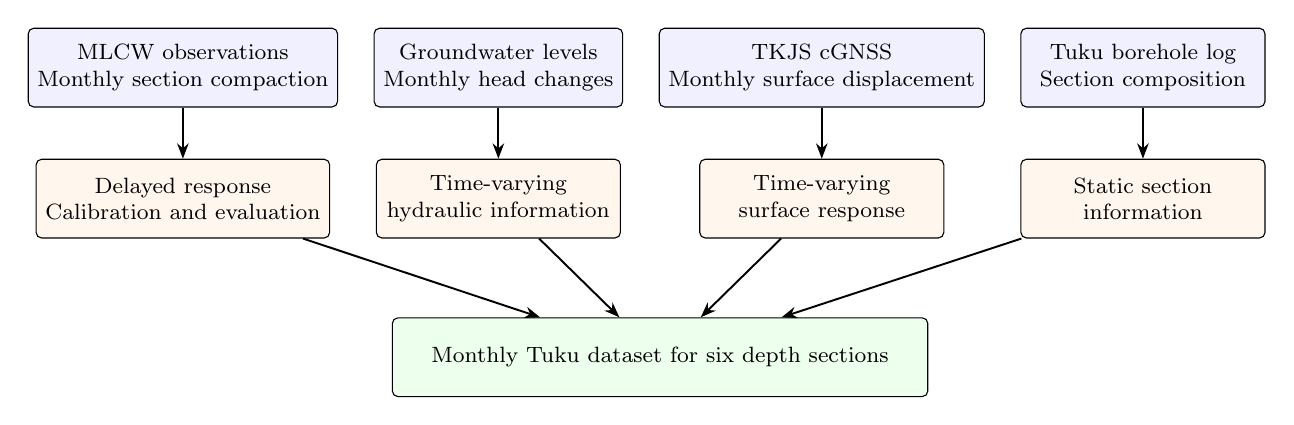
\begin{tikzpicture}[
    node distance=0.65cm and 0.45cm,
    source/.style={draw, rectangle, rounded corners=2pt, align=center, fill=blue!6, minimum width=3.1cm, minimum height=1.0cm, font=\footnotesize},
    process/.style={draw, rectangle, rounded corners=2pt, align=center, fill=orange!7, minimum width=3.1cm, minimum height=1.0cm, font=\footnotesize},
    result/.style={draw, rectangle, rounded corners=2pt, align=center, fill=green!7, minimum width=6.8cm, minimum height=1.0cm, font=\footnotesize},
    arrow/.style={-{Stealth[scale=0.9]}, line width=0.7pt}
  ]
    \node (mlcw) [source] {MLCW observations\\Monthly section compaction};
    \node (gwl) [source, right=of mlcw] {Groundwater levels\\Monthly head changes};
    \node (gnss) [source, right=of gwl] {TKJS cGNSS\\Monthly surface displacement};
    \node (lith) [source, right=of gnss] {Tuku borehole log\\Section composition};

    \node (response) [process, below=of mlcw] {Delayed response\\Calibration and evaluation};
    \node (hydraulic) [process, below=of gwl] {Time-varying\\hydraulic information};
    \node (surface) [process, below=of gnss] {Time-varying\\surface response};
    \node (sediment) [process, below=of lith] {Static section\\information};

    \node (modeldata) [result, below=1.0cm of $(hydraulic.south)!0.5!(surface.south)$] {Monthly Tuku dataset for six depth sections};

    \draw [arrow] (mlcw) -- (response);
    \draw [arrow] (gwl) -- (hydraulic);
    \draw [arrow] (lith) -- (sediment);
    \draw [arrow] (gnss) -- (surface);
    \draw [arrow] (response) -- (modeldata);
    \draw [arrow] (hydraulic) -- (modeldata);
    \draw [arrow] (sediment) -- (modeldata);
    \draw [arrow] (surface) -- (modeldata);
  \end{tikzpicture}%
  }
  \caption{Integration of multilayer compaction, hydraulic head, vertical surface displacement, and sediment composition data for monthly section-level compaction estimation at Tuku.}
  \label{fig:tuku_data_workflow}
\end{figure}

\begin{table}[htbp]
  \centering
  \small
  \renewcommand{\arraystretch}{1.15}
  \caption{Datasets used for monthly compaction estimation at Tuku.}
  \label{tab:tuku_data_sources}
  \begin{tabularx}{\textwidth}{@{}>{\raggedright\arraybackslash}p{0.15\textwidth}>{\raggedright\arraybackslash}p{0.18\textwidth}>{\raggedright\arraybackslash}p{0.12\textwidth}>{\raggedright\arraybackslash}p{0.18\textwidth}>{\raggedright\arraybackslash}X@{}}
    \toprule
    \textbf{Dataset} & \textbf{Station or profile} & \textbf{Sampling interval} & \textbf{Observation period} & \textbf{Role in the analysis} \\
    \midrule
    MLCW compaction & Tuku MLCW, 0--300~m & Monthly & 01/2010--12/2024 & Monthly reference compaction for six depth sections \\
    Groundwater level & Tuku wells, Aquifers 1--4 & Daily & 01/2008--12/2024 & Monthly hydraulic head changes \\
    cGNSS displacement & TKJS & Daily & 01/2010--12/2024 & Monthly vertical surface displacement increments \\
    Borehole lithology & Tuku borehole, 0--300~m & Static & -- & Sediment composition within each depth section \\
    \bottomrule
  \end{tabularx}
\end{table}

\FloatBarrier


\section{Methodology}
\label{sec:methodology}
The analysis converted MLCW deformation, cGNSS displacement, and hydraulic head records into monthly variables. Separate Bayesian ridge regression models then related each section's monthly deformation increments to hydraulic head changes, vertical surface displacement, and seasonal variation. The estimates were evaluated under three monitoring conditions that differed in when, or whether, new MLCW observations became available. These conditions included temporary delays in finalized monthly records, reduced measurement schedules with one cumulative observation every six or twelve months, and the absence of subsequent MLCW measurements after an initial calibration period.

\subsection{Preparation of model inputs}
\label{subsec:predictor_preparation}

Model-input preparation began by aligning the MLCW and cGNSS displacement records, which were collected on different dates. A deformation time series model evaluated these records at common monthly dates and produced monthly increments. The MLCW increments formed the response, while cGNSS increments, section-specific hydraulic head changes, and seasonal terms formed the predictors.

\subsubsection{Deformation time series model}
\label{subsec:deformation_model}

For each MLCW and cGNSS displacement series, the deformation time series model represented displacement as the sum of a reference value, a linear component, annual and semiannual components, and offsets at documented discontinuities. For observation time $t$, the fitted displacement was
\begin{equation}
d(t)=d_0+v(t-t_0)
+\sum_{h\in\{1,2\}}
\left[a_h\sin(2\pi h t)+b_h\cos(2\pi h t)\right]
+\sum_{j=1}^{J}c_j H(t-t_j),
\label{eq:deformation_model}
\end{equation}
\noindent where $d_0$ denotes displacement at reference time $t_0$, $v$ denotes linear velocity, $a_h$ and $b_h$ describe the periodic components, and $H(t-t_j)$ represents a step at discontinuity time $t_j$ \citep{nikolaidis_observation_2002, bevis_2014}. The fitted series were evaluated at common monthly epochs to produce aligned cumulative displacement records. For depth section $s$, the deformation increment over the month ending at epoch $k$ was

\begin{equation}
\Delta d_{s,k}
=
d_s(t_k)-d_s(t_{k-1}),
\label{eq:monthly_deformation_increment}
\end{equation}

\noindent where $t_k$ and $t_{k-1}$ denote consecutive monthly epochs. Corresponding differences in the cGNSS series yielded monthly vertical surface displacement increments.

\subsubsection{Assembly of monthly model inputs}

Each observation in the regression dataset represented one depth section during one month, with the observed deformation increment $\Delta d_{s,k}$ serving as the response. The predictors described hydraulic conditions, vertical surface displacement, and seasonal variation.

Hydraulic head observations from the Tuku wells were used directly for the depth sections represented by local records. For the remaining sections, hydraulic head at Tuku was estimated from the regional monitoring network using ordinary kriging \citep{theodossiou2006}. Current and lagged hydraulic head changes from the target section and the other five sections were then included as candidate predictors to represent hydraulic conditions throughout the monitored profile. Concurrent and lagged cGNSS increments described vertical surface displacement, while annual, semiannual, and dry-season indicator terms represented recurring seasonal variation, including a dry-season interaction with hydraulic head change. Each section model used 38 input variables derived from hydraulic head, vertical surface displacement, and seasonal variation.

A separate calibration dataset was prepared for each depth section, and an independent regression model was fitted to each dataset. Before each six-month evaluation block, predictor centering and scaling were calculated only from the observations available for calibration and were subsequently applied to the evaluation block. Previous MLCW deformation increments were not used as predictors. \Cref{tab:predictor_summary} summarizes the information represented by each predictor group, whereas \Cref{app:predictors} provides the complete predictor definitions, data sources, temporal transformations, and lag periods.

\begin{table}[htbp]
  \centering
  \small
  \renewcommand{\arraystretch}{1.15}
  \caption{Predictor groups used to estimate monthly deformation increments at Tuku.}
  \label{tab:predictor_summary}
  \begin{tabularx}{\textwidth}{@{}p{0.21\textwidth}p{0.27\textwidth}X@{}}
    \toprule
    \textbf{Predictor group} & \textbf{Information represented} & \textbf{Role in the model} \\
    \midrule
    cGNSS displacement & Current and lagged vertical surface displacement increments & Described the integrated vertical response at Tuku \\
    Target-section hydraulic head & Current and lagged hydraulic head changes for the target section & Described hydraulic conditions associated with the section being estimated \\
    Other-section hydraulic head & Current and lagged hydraulic head changes for the other five depth sections & Included as candidate predictors representing system-wide hydraulic conditions \\
    Seasonal terms & Annual and semiannual variation & Represented recurring seasonal patterns \\
    \bottomrule
  \end{tabularx}
\end{table}

\subsection{Bayesian ridge regression}
\label{subsec:bayesian_ridge}

Bayesian ridge regression was used as a probabilistic linear regression model to estimate monthly deformation increments independently for each depth section. The predictors included current and lagged changes in hydraulic head and vertical surface displacement, together with seasonal terms. Several of these predictors described related temporal variations and therefore contained overlapping information. Under these conditions, ordinary least squares may produce regression coefficients that change markedly in response to small changes in the calibration data. Ridge regression limits this sensitivity by reducing the magnitude of coefficients that are weakly supported by the observations \citep{hoerl_1970_ridge}.

The Bayesian formulation applies the same coefficient shrinkage but also represents the remaining uncertainty in the fitted relation \citep{mackay_bayesian_1992}. For $n$ calibration observations and $p$ standardized predictors, the regression model was

\begin{equation}
\Delta\boldsymbol{d}_s
=
\beta_{0,s}\boldsymbol{1}
+
\boldsymbol{X}_s\boldsymbol{\beta}_s
+
\boldsymbol{\varepsilon}_s,
\label{eq:brr_regression}
\end{equation}

\noindent with residual errors described by

\begin{equation}
\boldsymbol{\varepsilon}_s
\sim
\mathcal{N}
\left(
\boldsymbol{0},
\alpha_s^{-1}\boldsymbol{I}
\right),
\label{eq:brr_likelihood}
\end{equation}

\noindent Here, $\Delta\boldsymbol{d}_s$ contains the observed monthly deformation increments for section $s$, $\beta_{0,s}$ is the intercept, $\boldsymbol{X}_s$ contains the standardized predictors, and $\boldsymbol{\beta}_s$ contains their regression coefficients. The residual term $\boldsymbol{\varepsilon}_s$ represents variation in monthly deformation that was not explained by the predictors. The parameter $\alpha_s$ describes the precision of this residual variation. A larger value of $\alpha_s$ corresponds to less unexplained variation around the fitted relation.

Coefficient shrinkage was introduced by assigning a zero-centered Gaussian distribution to the regression coefficients,

\begin{equation}
\boldsymbol{\beta}_s
\sim
\mathcal{N}
\left(
\boldsymbol{0},
\lambda_s^{-1}\boldsymbol{I}
\right),
\label{eq:brr_prior}
\end{equation}

\noindent where $\lambda_s$ controls the strength of the shrinkage for section $s$. A larger value of $\lambda_s$ pulls weakly supported coefficients more strongly toward zero, whereas predictors that are consistently related to monthly deformation have larger coefficients. The values of $\alpha_s$ and $\lambda_s$ were estimated from the calibration data by maximizing the marginal likelihood \citep{mackay_bayesian_1992}. In practical terms, this procedure allowed the observed record to determine both the unexplained variation and the degree of coefficient shrinkage.

Conventional ridge regression also reduces unstable coefficients, but it generally provides one fitted set of coefficients for a selected penalty. Bayesian ridge regression additionally describes a range of plausible coefficient values after the calibration data have been considered. This posterior distribution provides the information needed to quantify uncertainty in subsequent monthly estimates.

A separate model was fitted for each depth section. Thus, the regression coefficients for a section were estimated only from its own MLCW deformation record, although its predictors could include hydraulic head changes from other sections of the monitored profile. The fitted relations were interpreted as statistical associations within the Tuku monitoring record and not as a substitute for a coupled groundwater flow and aquifer-system compaction model.

\subsection{Predictive uncertainty quantification}
\label{subsec:predictive_uncertainty}

The Bayesian formulation provided both a monthly deformation estimate and a measure of uncertainty around that estimate. This uncertainty was represented by the posterior predictive distribution, which combines variation not explained by the regression model with uncertainty in the fitted regression coefficients \citep{mackay_bayesian_1992}. For a new monthly epoch with standardized predictors $\boldsymbol{x}_{s,*}$ and calibration data $\mathcal{D}_s$, the posterior predictive distribution for section $s$ was

\begin{equation}
p
\left(
\Delta d_{s,*}
\mid
\boldsymbol{x}_{s,*},
\mathcal{D}_s
\right)
=
\mathcal{N}
\left(
\mu_{s,*},
\sigma_{s,*}^{2}
\right).
\label{eq:posterior_predictive}
\end{equation}

Its predictive mean was

\begin{equation}
\mu_{s,*}
=
\widehat{\beta}_{0,s}
+
\boldsymbol{x}_{s,*}^{\mathsf{T}}
\overline{\boldsymbol{\beta}}_s,
\label{eq:predictive_mean}
\end{equation}

The corresponding point estimate was

\begin{equation}
\widehat{\Delta d}_{s,*}
=
\mu_{s,*}.
\label{eq:monthly_deformation_estimate}
\end{equation}

The predictive variance was

\begin{equation}
\sigma_{s,*}^{2}
=
\alpha_s^{-1}
+
\boldsymbol{x}_{s,*}^{\mathsf{T}}
\boldsymbol{\Sigma}_{\beta,s}
\boldsymbol{x}_{s,*}.
\label{eq:predictive_variance}
\end{equation}

\noindent Here, $\widehat{\beta}_{0,s}$ is the fitted intercept, $\overline{\boldsymbol{\beta}}_s$ is the posterior mean of the regression coefficients, and $\boldsymbol{\Sigma}_{\beta,s}$ is their posterior covariance matrix. The first term in the predictive variance represents residual variation that was not explained by the model. The second term represents uncertainty in the fitted coefficients for the corresponding predictor values. The predictive interval therefore became wider when the residual variation was larger or when the coefficients were less strongly constrained by the calibration data.

The nominal 90\% posterior predictive interval was calculated as

\begin{equation}
\left[
\mu_{s,*}-1.645\sigma_{s,*},
\mu_{s,*}+1.645\sigma_{s,*}
\right],
\label{eq:prediction_interval}
\end{equation}

This interval described the range of monthly deformation increments considered plausible under the fitted model. Because it was calculated directly from the posterior predictive distribution, an interval was available for every monthly estimate without requiring an archive of previous prediction errors.

Interval performance was evaluated using empirical coverage and mean interval width. Empirical coverage measured the proportion of observed monthly increments enclosed by the intervals. Mean interval width described how broadly the plausible values were distributed around the monthly estimates. Both measures were examined because a wider interval may enclose more observations while providing less precise information \citep{singh_uncertainty_2024}. The nominal 90\% level provided a reference for this evaluation, but it did not guarantee that exactly 90\% of the observations would be enclosed. Temporal dependence and relations not represented by the regression model could cause the empirical coverage to differ from the nominal level.

\subsection{Experimental design}
\label{subsec:experimental_design}

All three evaluation designs preserved the temporal order of the monitoring records. For each period being estimated, the model used only MLCW observations that would have been available before that period, while monthly GWL and cGNSS observations remained available during the estimation period. This design prevented later MLCW observations from influencing earlier estimates. The three evaluations differed in when, or whether, new MLCW observations became available for updating the model.

\subsubsection{Monthly estimation with delayed MLCW records}
\label{subsec:delayed_evaluation}

Temporary gaps in the availability of finalized monthly MLCW records were examined using a recurring estimation and update cycle. The model was first calibrated using three years of continuous monthly observations. During each subsequent six-month period, the available GWL and cGNSS observations were used to estimate monthly deformation increments while the corresponding MLCW observations remained unavailable. The six-month interval provided a consistent basis for comparison and did not represent a fixed schedule for data provision.

At the end of each estimation period, the corresponding monthly MLCW observations became available and were compared with the estimates. These observations were then added to the calibration record, after which the model was recalibrated for the next cycle. Repeating this sequence gradually expanded the calibration record while preserving temporal order because observations from a later period could not influence earlier estimates. One complete cycle is illustrated in \Cref{fig:delayed_observation_design}.

Point estimates were evaluated separately for each depth section and for all sections combined using the coefficient of determination ($R^2$), root mean square error (RMSE), and mean absolute error (MAE). Posterior predictive intervals were evaluated using empirical coverage and mean interval width, as described in \Cref{subsec:predictive_uncertainty}. Performance was also compared across successive months within each update cycle to determine whether estimation quality changed as the MLCW observation gap lengthened.

\begin{figure}[htbp]
  \centering
  \resizebox{\linewidth}{!}{%
  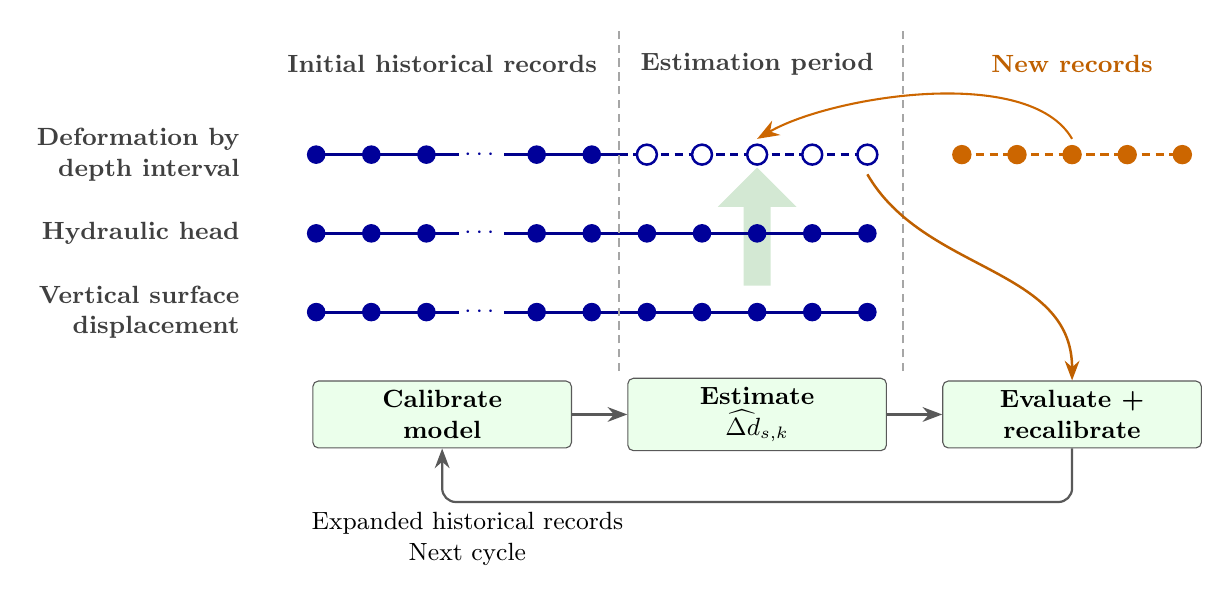
\begin{tikzpicture}[
    font=\small,
    dataset/.style={anchor=east,align=right,font=\small\bfseries,text=black!75},
    phase/.style={font=\small\bfseries,text=black!75,align=center},
    updatephase/.style={font=\small\bfseries,text=orange!75!black,align=center},
    available/.style={circle,draw=blue!60!black,fill=blue!60!black,minimum size=6.3pt,inner sep=0pt},
    pending/.style={circle,draw=blue!60!black,fill=white,line width=0.9pt,minimum size=7.2pt,inner sep=0pt},
    newrecord/.style={circle,draw=orange!80!black,fill=orange!80!black,minimum size=6.6pt,inner sep=0pt},
    historyline/.style={draw=blue!55!black,line width=1.1pt},
    pendingline/.style={draw=blue!55!black,densely dashed,line width=0.9pt},
    divider/.style={draw=black!35,densely dashed,line width=0.7pt},
    flow/.style={-{Stealth[length=2.5mm]},draw=black!65,line width=0.8pt},
    orangeflow/.style={-{Stealth[length=2.5mm]},draw=orange!75!black,line width=0.9pt},
    orangeline/.style={draw=orange!80!black,densely dashed,line width=1.1pt},
    curvedflow/.style={-{Stealth[length=2.8mm]},draw=orange!80!black,line width=0.75pt},
    fadedarrow/.style={
      single arrow,
      draw=none,
      fill={rgb,255:red,34;green,139;blue,34},
      fill opacity=0.2,
      shape border rotate=90,
      minimum height=1.5cm,
      minimum width=1.0cm,
      single arrow head extend=0.8mm,
      inner sep=1pt
    },
    action/.style={draw=black!65,fill=green!8,rounded corners=2pt,align=center,minimum height=0.85cm,text width=3.05cm,font=\small\bfseries}
  ]
    \node[phase] at (2.00,3.70) {Initial historical records};
    \node[phase] at (6.00,3.70) {Estimation period};
    \node[updatephase] at (10.00,3.70) {New records};

    \node[dataset] at (-0.45,2.55) {Deformation by\\depth interval};
    \node[dataset] at (-0.45,1.55) {Hydraulic head};
    \node[dataset] at (-0.45,0.55) {Vertical surface\\displacement};

    \node[fadedarrow] at (6.00,1.55) {};

    \foreach \y in {1.55,0.55} {
      \draw[historyline] (0.40,\y) -- (7.40,\y);
    }
    \draw[historyline] (0.40,2.55) -- (4.25,2.55);
    \draw[pendingline] (4.25,2.55) -- (7.40,2.55);

    \foreach \y in {2.55,1.55,0.55} {
      \foreach \x in {0.40,1.10,1.80,3.20,3.90} {
        \node[available] at (\x,\y) {};
      }
      \node[fill=white,inner xsep=2pt,text=blue!60!black] at (2.50,\y) {$\cdots$};
    }

    \foreach \y in {1.55,0.55} {
      \foreach \x in {4.60,5.30,6.00,6.70,7.40} {
        \node[available] at (\x,\y) {};
      }
    }

    \foreach \x in {4.60,5.30,6.00,6.70,7.40} {
      \node[pending] at (\x,2.55) {};
    }

    \draw[orangeline] (8.60,2.55) -- (11.40,2.55);
    \foreach \x in {8.60,9.30,10.00,10.70,11.40} {
      \node[newrecord] at (\x,2.55) {};
    }

    \draw[curvedflow] (10.00,2.75) to[out=120,in=30,looseness=0.7] (6.00,2.75);

    \draw[divider] (4.25,-0.2) -- (4.25,4.15);
    \draw[divider] (7.85,-0.2) -- (7.85,4.15);

    \node[action] (calibrate) at (2.00,-0.75) {Calibrate\\model};
    \node[action] (estimate) at (6.00,-0.75) {Estimate\\$\widehat{\Delta d}_{s,k}$};
    \node[action] (update) at (10.00,-0.75) {Evaluate +\\recalibrate};
    \draw[flow] (calibrate.east) -- (estimate.west);
    \draw[flow] (estimate.east) -- (update.west);
    \draw[orangeflow] (7.4,2.3) to[out=-60,in=90] (update.north);
    \draw[flow,rounded corners=5pt]
      (update.south) -- ++(0,-0.68) -| (calibrate.south)
      node[pos=0.48,below,align=center,font=\small]
      {Expanded historical records\\Next cycle};
  \end{tikzpicture}%
  }
  \caption{Estimation and model updating during the temporary unavailability of finalized monthly depth-interval deformation records. Hydraulic head and vertical surface displacement remained available during this period. Filled blue markers denote available observations, open blue markers denote deformation records not yet available, and orange markers denote the records subsequently provided. The symbol $\widehat{\Delta d}_{s,k}$ denotes the estimated monthly deformation increment for section $s$. Dots indicate omitted records; marker counts and spacing are illustrative.}
  \label{fig:delayed_observation_design}
\end{figure}

\subsubsection{Sensitivity to less frequent MLCW field measurements}
\label{subsec:sparse_measurement_sensitivity}

Reduced MLCW measurement frequency was examined under hypothetical schedules in which MLCW observations became available only at the end of each measurement interval. Monthly GWL and cGNSS observations remained available throughout the interval and were used to estimate monthly deformation increments. The intervening monthly MLCW values were excluded from estimation and model updating, and one cumulative MLCW deformation observation became available at the interval endpoint.

The evaluated scenarios combined measurement intervals of 6 or 12 months with initial calibration periods containing 36, 60, or 96 consecutive monthly MLCW observations. All three calibration periods ended on the same calendar date, so the 36- and 60-month periods began later than the 96-month period rather than starting from the same date and ending earlier. This shared calibration endpoint let the three initial-history lengths be compared over an identical subsequent record rather than over three different sets of calendar months. Each measurement schedule was then evaluated over an identical subsequent period, ending at a shared field-measurement date, so that the three initial-history lengths underwent the same number of model updates at the same calendar dates within a given measurement schedule. Because a 6-month schedule and a 12-month schedule complete different numbers of measurement intervals over the same period, the two schedules were compared using their own respective update counts rather than a common count; only the initial-history-length comparison required matching update counts and dates. These durations defined the scenarios examined in this study rather than a requirement of the method. Regardless of the selected duration, each measurement interval produced one cumulative deformation observation.

To represent this cumulative observation mathematically, let $s$ denote a depth section, $k$ denote a monthly epoch, $I$ denote a measurement interval, and $H_I$ denote the number of months in that interval. The observed monthly MLCW deformation increment is denoted by $\Delta d_{s,k}$, as defined in \Cref{eq:monthly_deformation_increment}. The cumulative deformation observed over interval $I$ was

\begin{equation}
\Delta d_{s,I}
=
\sum_{k\in I}\Delta d_{s,k}.
\label{eq:cumulative_deformation_observation}
\end{equation}

The individual monthly values within $I$ remained hidden from model fitting and updating and were used only for retrospective evaluation. Consequently, only the cumulative observation $\Delta d_{s,I}$ entered the next model update. Representing this observation within the monthly regression required the relation in \Cref{eq:brr_regression,eq:brr_likelihood} to be accumulated over the same interval. This summation gave

\begin{equation}
\Delta d_{s,I}
=
H_I\beta_{0,s}
+
\left(
\sum_{k\in I}\boldsymbol{x}_{s,k}
\right)^{\mathsf{T}}
\boldsymbol{\beta}_{s}
+
\varepsilon_{s,I},
\label{eq:cumulative_deformation_model}
\end{equation}

\noindent where $\boldsymbol{x}_{s,k}$ contains the standardized predictors for section $s$ at monthly epoch $k$, and $\varepsilon_{s,I}$ is the sum of the monthly residuals within the interval. This cumulative equation assumed that the monthly relation between the predictors and deformation remained unchanged between successive model updates. It also preserved the residual model in \Cref{eq:brr_likelihood}, under which the monthly residuals were independent, normally distributed around zero, and described by a constant variance within each depth section. Their variances therefore accumulated over the measurement interval, and the cumulative residual followed

\begin{equation}
\varepsilon_{s,I}
\sim
\mathcal{N}
\left(
0,
H_I\alpha_s^{-1}
\right).
\label{eq:cumulative_residual_distribution}
\end{equation}

The resulting variance increased in proportion to $H_I$. To fit the cumulative observation together with the original monthly observations, both observation types were placed on the same residual variance scale. The monthly predictors were first centered and scaled using only the initial monthly calibration record. The cumulative regression equation was then divided by $\sqrt{H_I}$,

\begin{equation}
\frac{\Delta d_{s,I}}{\sqrt{H_I}}
=
\sqrt{H_I}\,\beta_{0,s}
+
\left(
\frac{1}{\sqrt{H_I}}
\sum_{k\in I}\boldsymbol{x}_{s,k}
\right)^{\mathsf{T}}
\boldsymbol{\beta}_{s}
+
\widetilde{\varepsilon}_{s,I},
\label{eq:scaled_cumulative_deformation_model}
\end{equation}

\noindent with

\begin{equation}
\widetilde{\varepsilon}_{s,I}
=
\frac{\varepsilon_{s,I}}{\sqrt{H_I}}
\sim
\mathcal{N}
\left(
0,
\alpha_s^{-1}
\right).
\label{eq:scaled_cumulative_residual}
\end{equation}

This scaling did not divide the cumulative observation into separate monthly measurements. Instead, it allowed the monthly and cumulative observations to constrain the same regression coefficients while preserving their different temporal support. The scaled cumulative equation could therefore enter the calibration record as one interval constraint.

The model was first calibrated from the initial monthly MLCW record and used to estimate deformation throughout the first measurement interval. At the end of that interval, the cumulative observation in \Cref{eq:cumulative_deformation_observation} was added to the calibration record as one interval constraint. The expanded record, consisting of the initial monthly observations and cumulative observations from completed intervals, was then used to recalibrate the model before the next interval. Hidden monthly MLCW values from the reduced measurement intervals never entered this recalibration. This sequence is illustrated in \Cref{fig:reduced_measurement_design}.

\begin{figure}[htbp]
  \centering
  \resizebox{\linewidth}{!}{%
  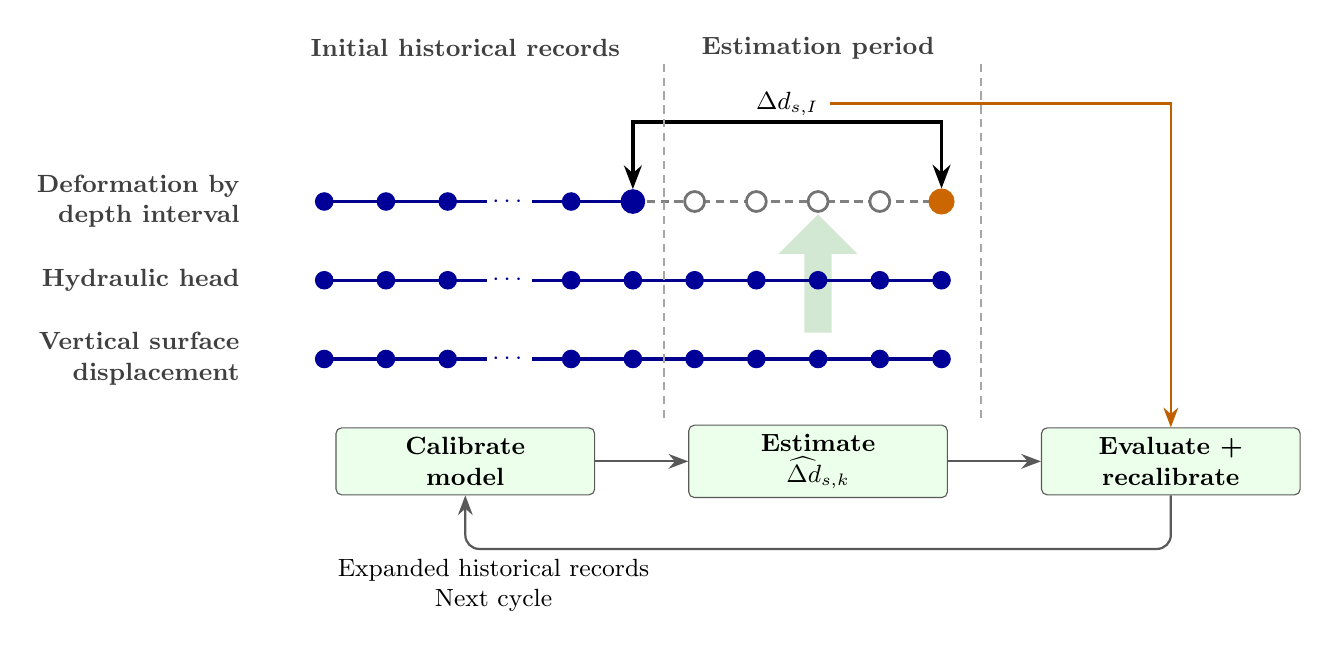
\begin{tikzpicture}[
    x=1.12cm,
    y=1cm,
    font=\small,
    dataset/.style={anchor=east,align=right,font=\small\bfseries,text=black!75},
    phase/.style={font=\small\bfseries,text=black!75,align=center},
    available/.style={circle,draw=blue!60!black,fill=blue!60!black,minimum size=6.3pt,inner sep=0pt},
    estimate/.style={circle,draw=black!55,fill=white,line width=1.0pt,minimum size=7.2pt,inner sep=0pt},
    startrecord/.style={circle,draw=blue!60!black,fill=blue!60!black,minimum size=8.5pt,inner sep=0pt},
    latestrecord/.style={circle,draw=orange!80!black,fill=orange!80!black,minimum size=9pt,inner sep=0pt},
    historyline/.style={draw=blue!55!black,line width=1.1pt},
    estimateline/.style={draw=black!50,densely dashed,line width=0.9pt},
    divider/.style={draw=black!35,densely dashed,line width=0.7pt},
    flow/.style={-{Stealth[length=2.5mm]},draw=black!65,line width=0.8pt},
    predictorflow/.style={-{Stealth[length=2.7mm]},draw=green!45!black,line width=1.15pt},
    orangeflow/.style={-{Stealth[length=2.5mm]},draw=orange!75!black,line width=0.9pt},
    toparrow/.style={{Stealth[length=3mm]}-{Stealth[length=3mm]},draw=black,line width=1.4pt},
    fadedarrow/.style={
      single arrow,
      draw=none,
      fill={rgb,255:red,34;green,139;blue,34},
      fill opacity=0.2,
      shape border rotate=90,
      minimum height=1.5cm,
      minimum width=1.0cm,
      single arrow head extend=0.8mm,
      inner sep=1pt
    },
    action/.style={draw=black!65,fill=green!8,rounded corners=2pt,align=center,minimum height=0.85cm,text width=3.05cm,font=\small\bfseries}
  ]
    \node[phase] at (2.00,4.5) {Initial historical records};
    \node[phase] at (6.00,4.5) {Estimation period};

    \node[dataset] at (-0.45,2.55) {Deformation by\\depth interval};
    \node[dataset] at (-0.45,1.55) {Hydraulic head};
    \node[dataset] at (-0.45,0.55) {Vertical surface\\displacement};

    \node[fadedarrow] at (6.00,1.55) {};

    \foreach \y in {1.55,0.55} {
      \draw[historyline] (0.40,\y) -- (7.40,\y);
    }
    \draw[historyline] (0.40,2.55) -- (3.90,2.55);
    \draw[estimateline] (3.90,2.55) -- (7.40,2.55);

    \foreach \y in {1.55,0.55} {
      \foreach \x in {0.40,1.10,1.80,3.20,3.90} {
        \node[available] at (\x,\y) {};
      }
      \node[fill=white,inner xsep=2pt,text=blue!60!black] at (2.50,\y) {$\cdots$};
    }
    \foreach \x in {0.40,1.10,1.80,3.20} {
      \node[available] at (\x,2.55) {};
    }
    \node[fill=white,inner xsep=2pt,text=blue!60!black] at (2.50,2.55) {$\cdots$};
    \node[startrecord] (start) at (3.90,2.55) {};

    \foreach \y in {1.55,0.55} {
      \foreach \x in {4.60,5.30,6.00,6.70,7.40} {
        \node[available] at (\x,\y) {};
      }
    }
    \foreach \x in {4.60,5.30,6.00,6.70} {
      \node[estimate] at (\x,2.55) {};
    }

    \node[latestrecord] (finish) at (7.40,2.55) {};

    \draw[toparrow]
      (start.north) -- ++(0,0.85) -| (finish.north)
      node[pos=0.25,above=-1.5pt,font=\small,text=black] (intervaldeformation)
      {$\Delta d_{s,I}$};

    \draw[divider] (4.25,-0.2) -- (4.25,4.35);
    \draw[divider] (7.85,-0.2) -- (7.85,4.35);

    \node[action] (calibrate) at (2.00,-0.75) {Calibrate\\model};
    \node[action] (estimatebox) at (6.00,-0.75) {Estimate\\$\widehat{\Delta d}_{s,k}$};
    \node[action] (update) at (10.00,-0.75) {Evaluate +\\recalibrate};
    \draw[flow] (calibrate.east) -- (estimatebox.west);
    \draw[flow] (estimatebox.east) -- (update.west);
    \draw[orangeflow] (intervaldeformation.east) -| (update.north);

    \draw[flow,rounded corners=5pt]
      (update.south) -- ++(0,-0.68) -| (calibrate.south)
      node[pos=0.48,below,align=center,font=\small]
      {Expanded historical records\\Next cycle};
  \end{tikzpicture}%
  }
  \caption{Monthly deformation estimation under reduced measurement frequency. Filled blue markers denote available observations, while hydraulic head and vertical surface displacement remained available monthly. Open gray markers denote monthly estimates $\widehat{\Delta d}_{s,k}$, and the blue and orange endpoints define the observed cumulative deformation $\Delta d_{s,I}$ over interval $I$. Dots indicate omitted records; marker counts and spacing are illustrative.}
  \label{fig:reduced_measurement_design}
\end{figure}

The resulting estimates were evaluated at monthly and interval scales. At the monthly scale, the error compared each estimated increment with its hidden monthly MLCW value,

\begin{equation}
e_{s,k}
=
\widehat{\Delta d}_{s,k}
-
\Delta d_{s,k}.
\label{eq:sparse_monthly_error}
\end{equation}

At the interval scale, the endpoint error compared the accumulated monthly estimates with the cumulative observation,

\begin{equation}
e_{s,I}
=
\sum_{k\in I}\widehat{\Delta d}_{s,k}
-
\Delta d_{s,I}.
\label{eq:sparse_endpoint_error}
\end{equation}

Monthly errors described how well the model distributed deformation within each interval, whereas endpoint errors described agreement with the cumulative field observation. Both error types were summarized using MAE, RMSE, and mean signed error for each depth section and for all sections combined. The coefficient of determination was not calculated for the endpoint observations because each scenario contained relatively few cumulative measurements.

\subsubsection{Sensitivity without subsequent MLCW field measurements}
\label{subsec:permanent_stoppage_sensitivity}

The absence of subsequent MLCW measurements was examined using models calibrated once from initial records spanning 3, 5, or 8 years. All three calibration records ended on the same calendar date, so the 3- and 5-year records began later than the 8-year record rather than starting from the same date and ending earlier. This shared calibration endpoint let the three initial-history lengths be compared over an identical subsequent record rather than over three different sets of calendar months. After each calibration record ended, monthly GWL and cGNSS observations continued to provide predictor values, but no later MLCW observations were added. The model coefficients and predictor scaling therefore remained fixed throughout the subsequent estimation period.

The remaining historical MLCW observations allowed this hypothetical condition to be evaluated retrospectively. These observations were withheld from model fitting and were used only to compare the observed monthly deformation increments with the estimates generated after the calibration record. The monthly error $e_{s,k}$ was calculated as defined in \Cref{eq:sparse_monthly_error}.

The accumulation of monthly errors was evaluated over the first $K$ months after calibration. The cumulative signed error for section $s$ was

\begin{equation}
E_{s,K}
=
\sum_{k=1}^{K} e_{s,k},
\label{eq:stoppage_cumulative_signed_error}
\end{equation}

and its absolute magnitude was

\begin{equation}
A_{s,K}
=
\left|E_{s,K}\right|.
\label{eq:stoppage_absolute_cumulative_error}
\end{equation}

The signed value $E_{s,K}$ indicated whether the accumulated estimates were above or below the observed cumulative deformation, whereas $A_{s,K}$ described the magnitude of this difference without regard to direction.

Monthly estimation performance through horizon $K$ was summarized separately using

\begin{equation}
\operatorname{MAE}_{s,K}
=
\frac{1}{K}
\sum_{k=1}^{K}
\left|e_{s,k}\right|,
\label{eq:stoppage_running_mae}
\end{equation}

and

\begin{equation}
\operatorname{RMSE}_{s,K}
=
\sqrt{
\frac{1}{K}
\sum_{k=1}^{K}
e_{s,k}^{2}
}.
\label{eq:stoppage_running_rmse}
\end{equation}

These measures described the typical magnitude of the monthly errors from the end of calibration through horizon $K$. They therefore complemented $A_{s,K}$, which described the difference between the estimated and observed cumulative deformation at that horizon.

To account for the increasing duration of the estimation period, the absolute cumulative error was also expressed per elapsed month as

\begin{equation}
R_{s,K}
=
\frac{A_{s,K}}{K}.
\label{eq:stoppage_horizon_normalized_error}
\end{equation}

The normalized value $R_{s,K}$ was interpreted together with $A_{s,K}$. Because positive and negative monthly errors could partly cancel within $E_{s,K}$, a decrease in $R_{s,K}$ did not necessarily indicate that the absolute cumulative error had stopped growing.

The frozen Bayesian ridge model also provided the posterior predictive interval defined in \Cref{subsec:predictive_uncertainty} for each monthly estimate. These intervals described uncertainty in individual monthly deformation increments throughout the estimation period. They were not accumulated into uncertainty bands for $E_{s,K}$ or $A_{s,K}$ because the dependence among prediction errors from successive months was not represented in the cumulative calculation.

Because the three calibration records shared the same endpoint, all three left the same 80 months for retrospective evaluation, over the identical subsequent calendar period. The complete fit-once evaluation is illustrated in \Cref{fig:no_subsequent_mlcw_design}.

\begin{figure}[htbp]
  \centering
  \resizebox{\linewidth}{!}{%
  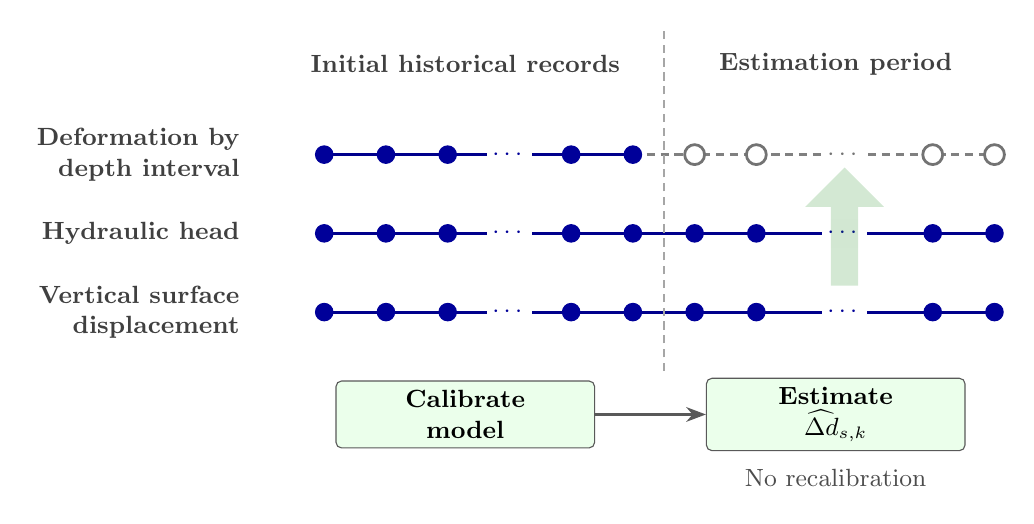
\begin{tikzpicture}[
  	x=1.12cm,
  	y=1cm,
  	font=\small,
  	dataset/.style={anchor=east,align=right,font=\small\bfseries,text=black!75},
  	phase/.style={font=\small\bfseries,text=black!75,align=center},
  	available/.style={circle,draw=blue!60!black,fill=blue!60!black,minimum size=6.3pt,inner sep=0pt},
  	estimate/.style={circle,draw=black!55,fill=white,line width=1.0pt,minimum size=7.2pt,inner sep=0pt},
  	historyline/.style={draw=blue!55!black,line width=1.1pt},
  	estimateline/.style={draw=black!50,densely dashed,line width=0.9pt},
  	divider/.style={draw=black!35,densely dashed,line width=0.7pt},
  	flow/.style={-{Stealth[length=2.5mm]},draw=black!65,line width=0.8pt},
  	fadedarrow/.style={
  		single arrow,
  		draw=none,
  		fill={rgb,255:red,34;green,139;blue,34},
  		fill opacity=0.2,
  		shape border rotate=90,
  		minimum height=1.5cm,
  		minimum width=1.0cm,
  		single arrow head extend=0.8mm,
  		inner sep=1pt
  	},
  	action/.style={draw=black!65,fill=green!8,rounded corners=2pt,align=center,minimum height=0.85cm,text width=3.05cm,font=\small\bfseries}
  	]
  	\node[phase] at (2.00,3.70) {Initial historical records};
  	\node[phase] at (6.20,3.70) {Estimation period};
  	
  	\node[dataset] at (-0.45,2.55) {Deformation by\\depth interval};
  	\node[dataset] at (-0.45,1.55) {Hydraulic head};
  	\node[dataset] at (-0.45,0.55) {Vertical surface\\displacement};
  	
  	% Continuous timelines
  	\foreach \y in {1.55,0.55} {
  		\draw[historyline] (0.40,\y) -- (8.00,\y);
  	}
  	\draw[historyline] (0.40,2.55) -- (3.90,2.55);
  	\draw[estimateline] (3.90,2.55) -- (8.00,2.55);
  	
  	% Panel 1 observations
  	\foreach \y in {2.55,1.55,0.55} {
  		\foreach \x in {0.40,1.10,1.80,3.20,3.90} {
  			\node[available] at (\x,\y) {};
  		}
  		\node[fill=white,inner xsep=2pt,text=blue!60!black] at (2.50,\y) {$\cdots$};
  	}
  	
  	% Panel 2 observations & dots
  	\foreach \y in {1.55,0.55} {
  		\foreach \x in {4.60,5.30,7.30,8.00} {
  			\node[available] at (\x,\y) {};
  		}
  		\node[fill=white,inner xsep=2pt,text=blue!60!black] at (6.30,\y) {$\cdots$};
  	}
  	\foreach \x in {4.60,5.30,7.30,8.00} {
  		\node[estimate] at (\x,2.55) {};
  	}
  	\node[fill=white,inner xsep=2pt,text=black!55] at (6.30,2.55) {$\cdots$};
  	
  	% CHUYỂN MŨI TÊN XANH XUỐNG ĐÂY VÀ ĐỔI SANG X=5.30
  	\node[fadedarrow] at (6.30,1.55) {};
  	
  	\draw[divider] (4.25,-0.2) -- (4.25,4.15);
  	
  	\node[action] (calibrate) at (2.00,-0.75) {Calibrate\\model};
  	\node[action] (estimatebox) at (6.20,-0.75) {Estimate\\$\widehat{\Delta d}_{s,k}$};
  	\draw[flow] (calibrate.east) -- (estimatebox.west);
  	\node[font=\small,text=black!70] at (6.20,-1.55) {No recalibration};
  \end{tikzpicture}
  }
  \caption{Fit-once monthly deformation estimation under the hypothetical absence of subsequent depth-interval deformation measurements. Filled blue markers denote observations used for model calibration. Hydraulic head and vertical surface displacement remained available, while open gray markers denote monthly estimates $\widehat{\Delta d}_{s,k}$. Model coefficients and predictor scaling remained fixed throughout the estimation period. Dots indicate omitted records; marker counts and spacing are illustrative.}
  \label{fig:no_subsequent_mlcw_design}
\end{figure}

\FloatBarrier


\section{Results}
\label{sec:results}
% Results. The earlier combined Results and Discussion draft remains available
% in results_discussion_draft.tex for comparison.

The three monitoring conditions differed in the availability of new MLCW information. Finalized monthly records became available after a temporary delay in one condition. The reduced-frequency condition provided one cumulative measurement every 6 or 12 months, whereas the final condition provided no subsequent MLCW measurement. The following subsections report how monthly and cumulative estimation errors changed across these conditions.

\subsection{Monthly estimation during delayed MLCW data delivery}
\label{subsec:results_delayed_delivery}

During delayed MLCW data delivery, estimated monthly increments followed the observed temporal patterns more closely in S1--S4 than in S5--S6. This comparison covered 23 complete six-month cycles from 05/2013 to 10/2024 and yielded 138 estimates for each depth section. After each cycle, the newly finalized monthly observations expanded the calibration record used for the next cycle (\Cref{fig:results_delayed_cycles}).

The monthly time series in \Cref{fig:results_delayed_monthly_estimates} show this contrast, and in \Cref{fig:results_delayed_scatter} the estimates for S1--S4 remained closer to the line of exact agreement than those for the two deepest sections.

\begin{figure}[htbp]
  \centering
  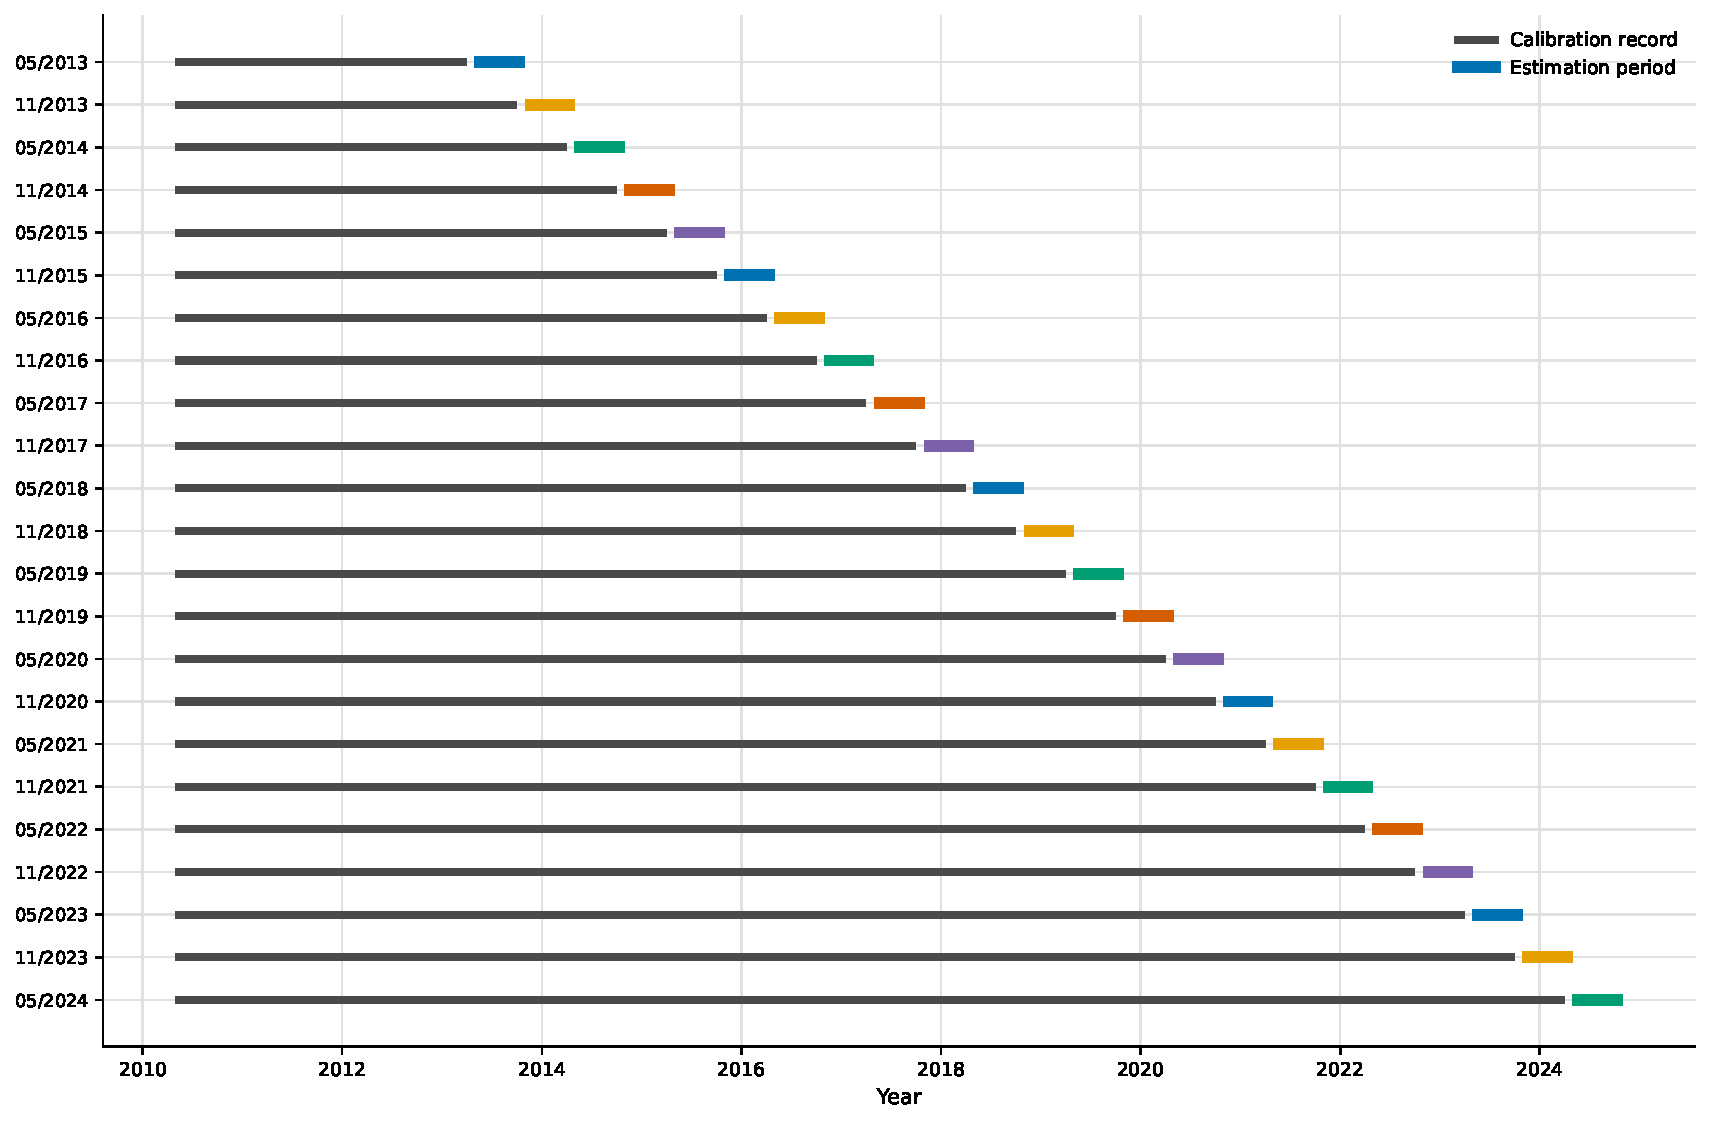
\includegraphics[width=0.98\textwidth]{figures/fig_results_delayed_cycle_timeline.pdf}
  \caption[Calibration and estimation periods during delayed MLCW data delivery.]{Successive calibration and estimation periods used to evaluate monthly deformation increments while finalized MLCW records were unavailable. The five colors repeat to distinguish adjacent estimation periods and do not represent different experimental conditions.}
  \label{fig:results_delayed_cycles}
\end{figure}

\begin{figure}[tp]
  \centering
  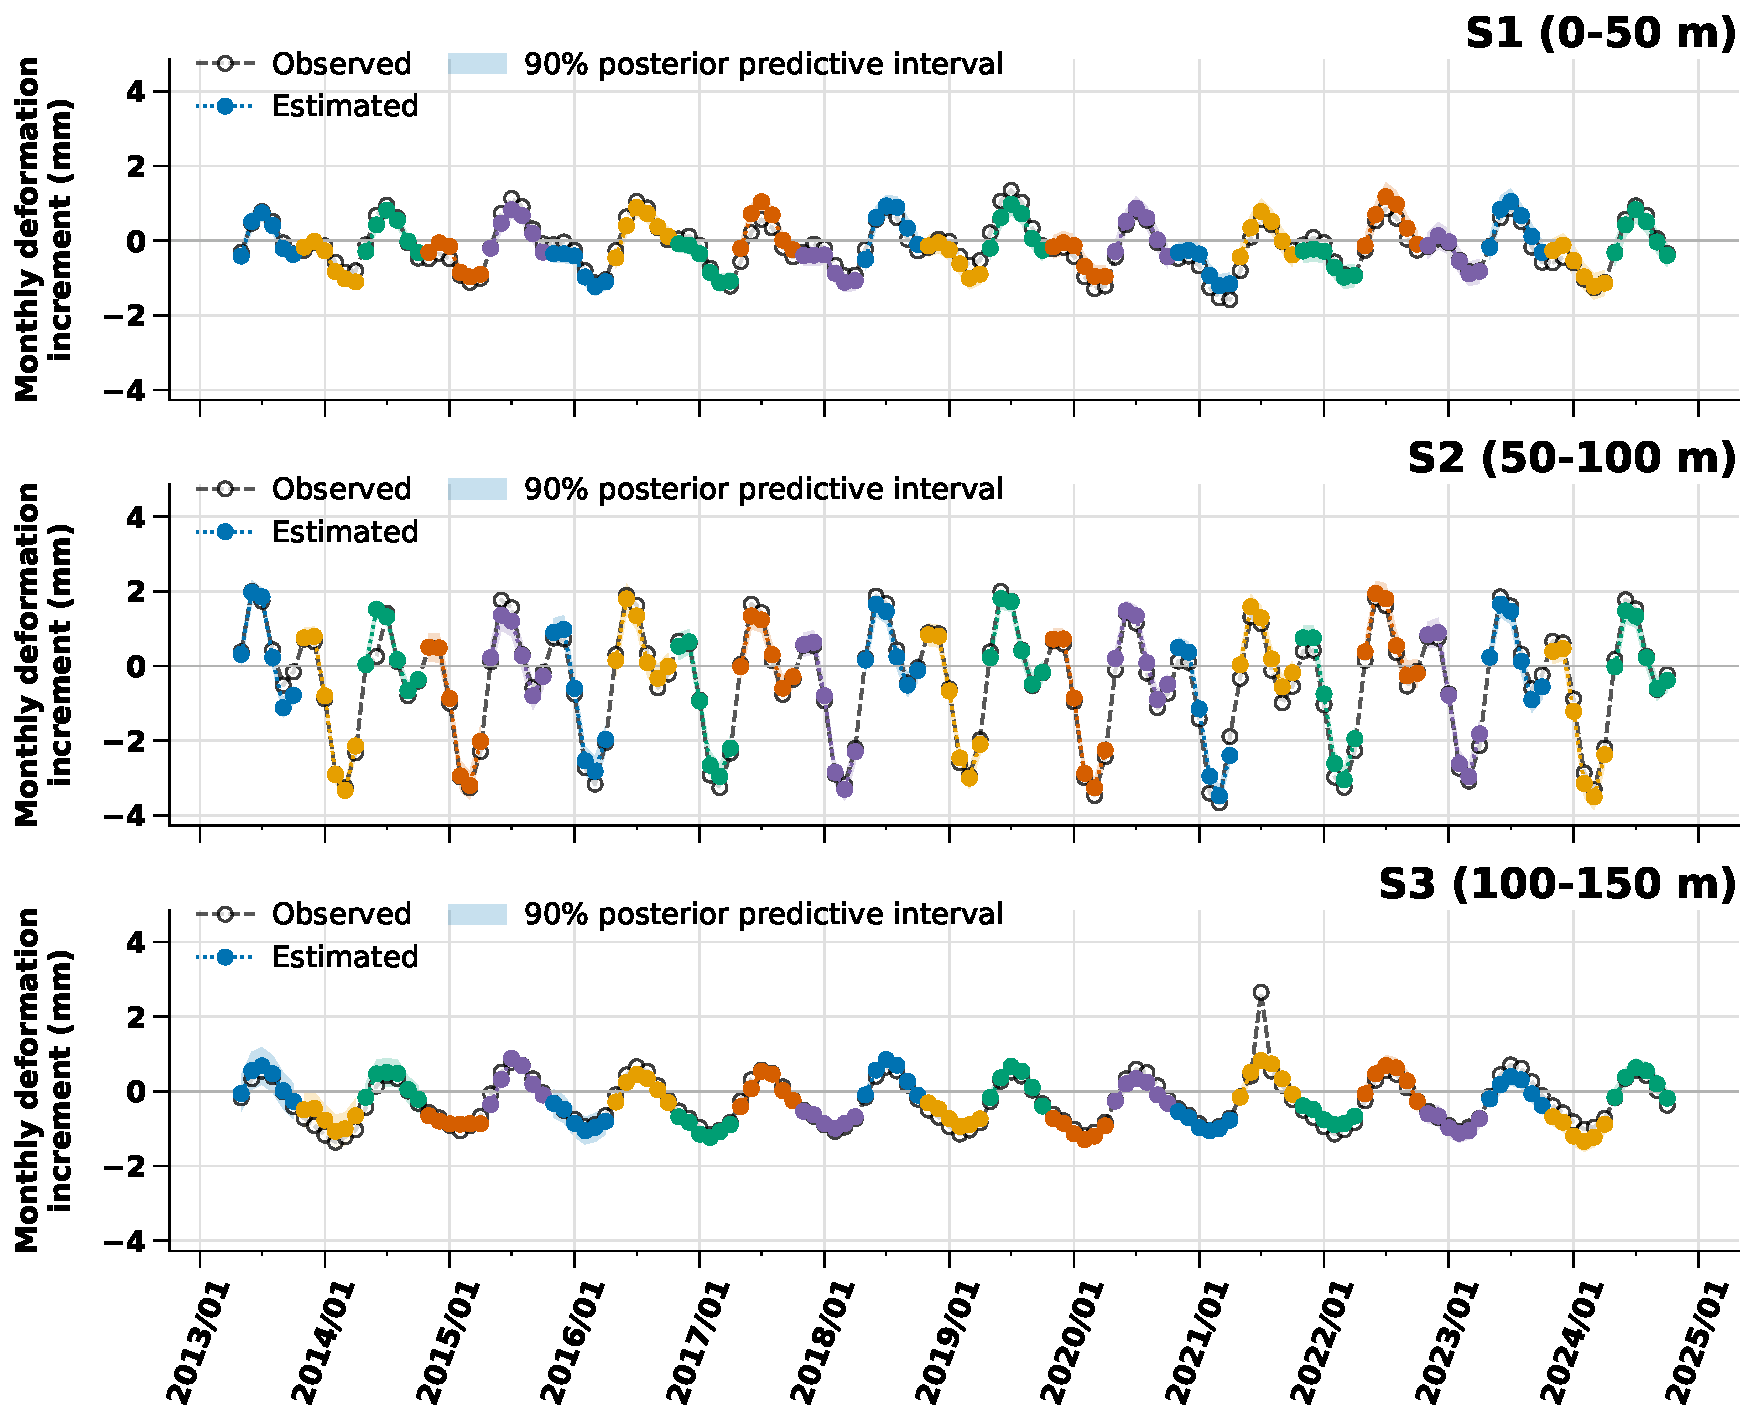
\includegraphics[width=0.98\textwidth]{figures/fig_results_delayed_monthly_estimates_s1_s3.pdf}
  \caption[Observed and estimated monthly deformation increments by depth section.]{Observed and estimated monthly deformation increments for S1--S3. The black lines show observations, colored dotted lines show estimates, and shaded bands show the 90\% Bayesian posterior predictive intervals, using the same repeating five-color scheme as \Cref{fig:results_delayed_cycles}.}
  \label{fig:results_delayed_monthly_estimates}
\end{figure}

\begin{figure}[tp]
  \ContinuedFloat
  \centering
  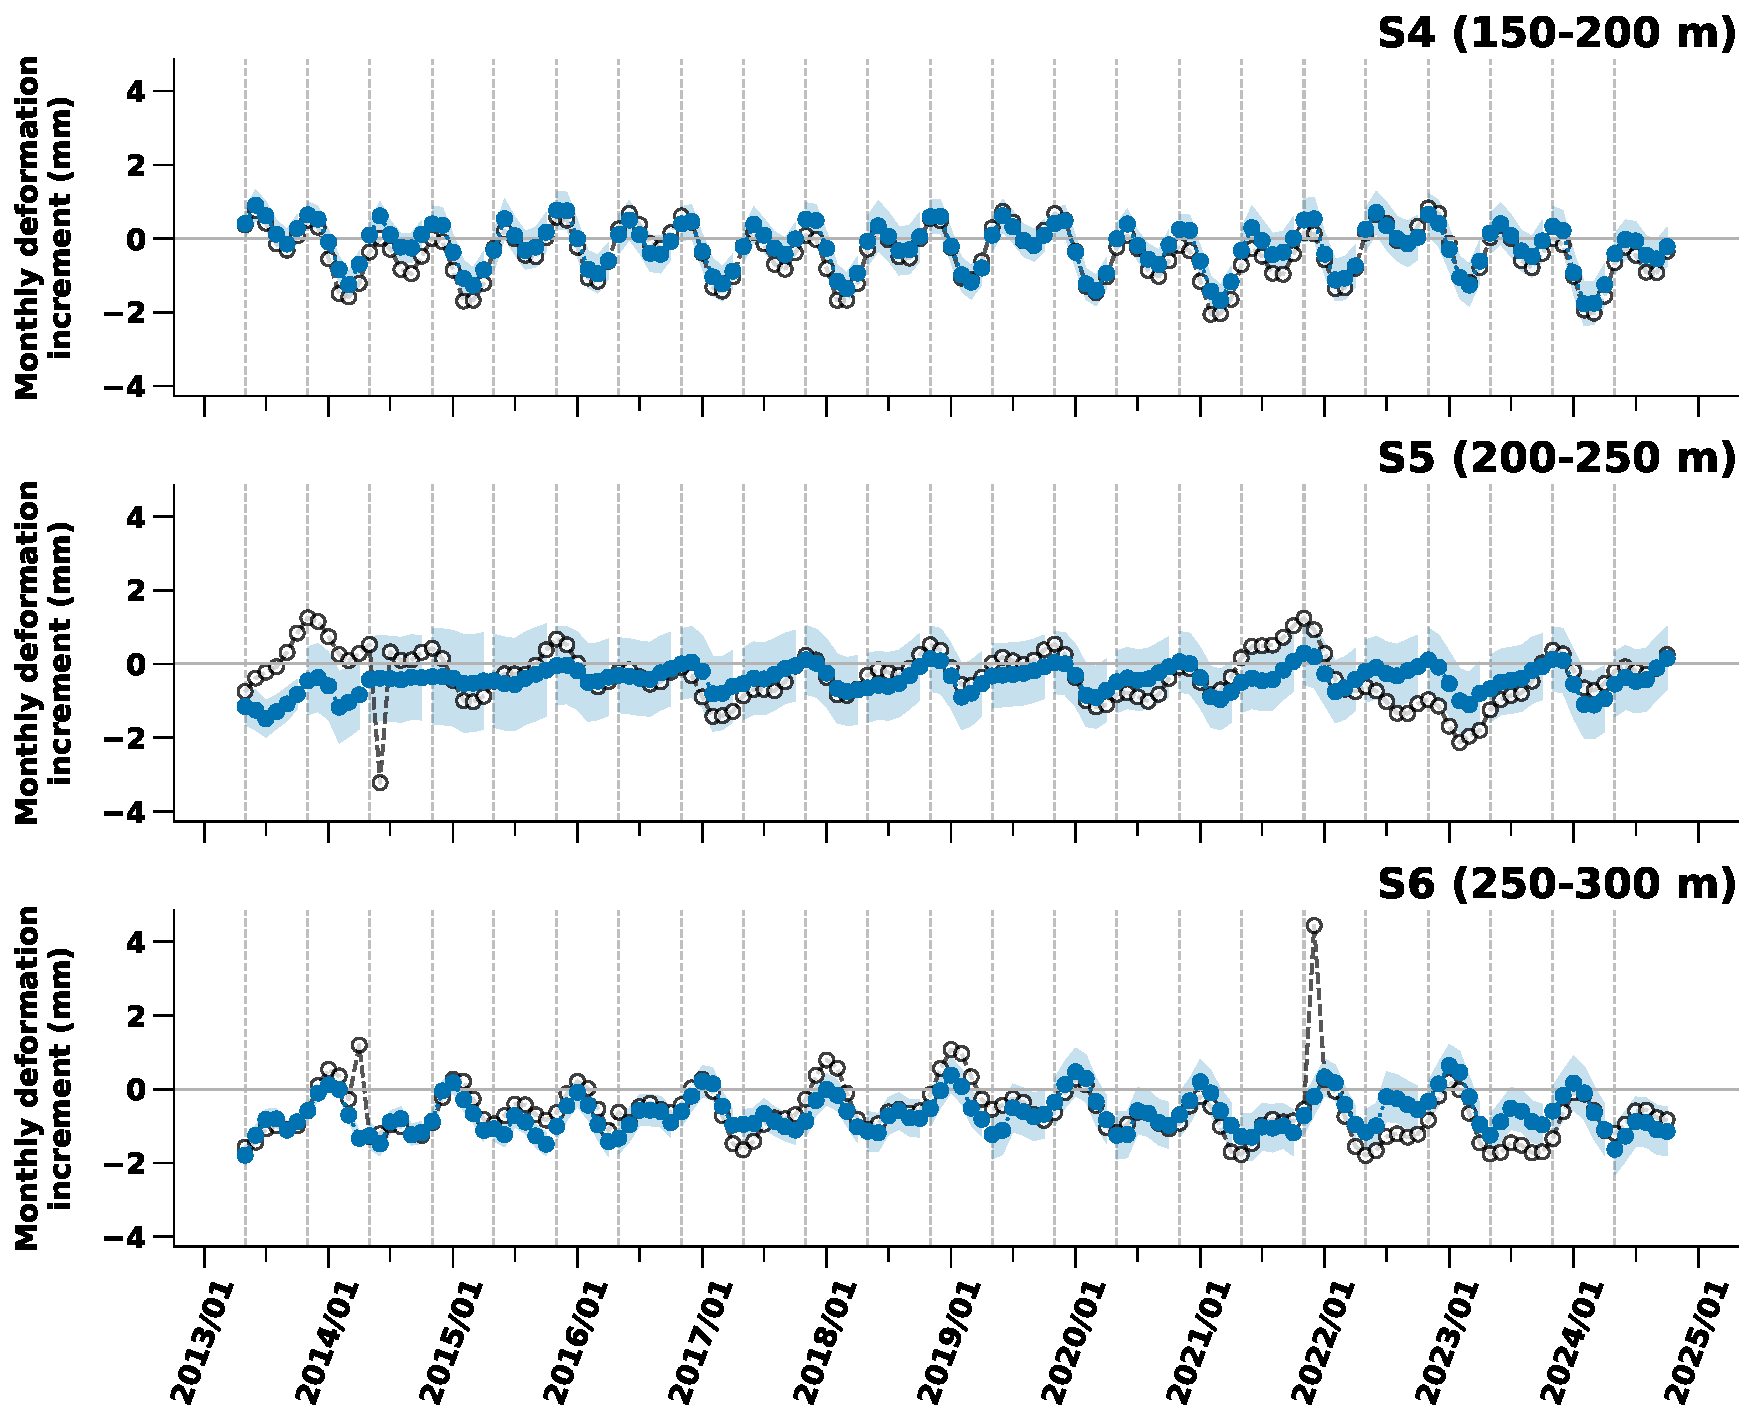
\includegraphics[width=0.98\textwidth]{figures/fig_results_delayed_monthly_estimates_s4_s6.pdf}
  \caption[]{Observed and estimated monthly deformation increments for S4--S6.}
\end{figure}

\begin{figure}[tp]
  \centering
  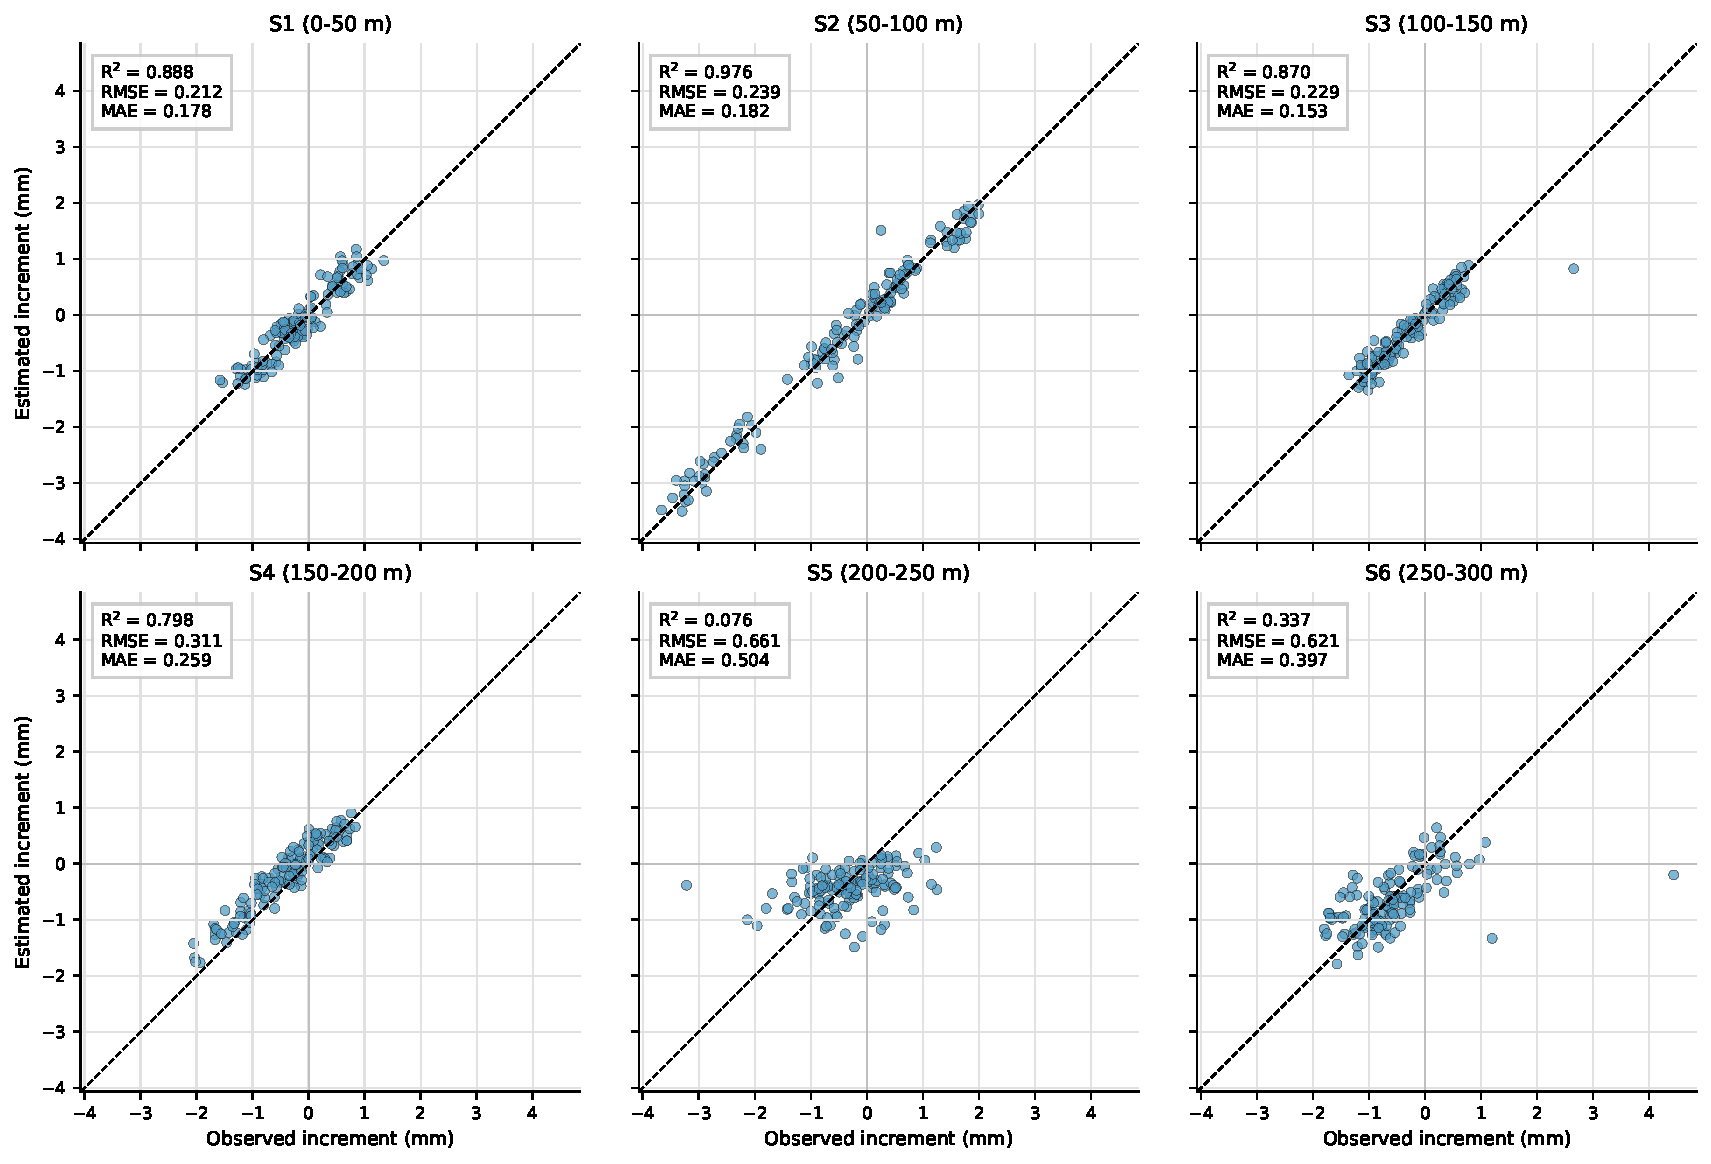
\includegraphics[width=0.98\textwidth]{figures/fig_results_delayed_prediction_vs_observed.pdf}
  \caption[Estimated versus observed monthly deformation increments.]{Estimated versus observed monthly deformation increments for the six depth sections. The dashed line represents exact agreement. RMSE and MAE are reported in mm/month.}
  \label{fig:results_delayed_scatter}
\end{figure}

\FloatBarrier

The depth contrast visible in the time series and scatter plots was also present in the error statistics (\Cref{tab:delayed_performance_interval}). Across the six depth sections, RMSE ranged from 0.21 to 0.66~mm/month and MAE ranged from 0.15 to 0.50~mm/month. Errors were smaller in S1--S4 than in S5 and S6, with S5 showing the largest RMSE and MAE.

The 90\% Bayesian posterior predictive intervals contained between 65.9\% and 88.4\% of the observations across the six sections, below the nominal 90\% level in every section, indicating the intervals were narrower than required. Possible sources of this gap are considered in \Cref{subsec:discussion_limitations}. Point-estimate error was worst in S5 and S6. Coverage, at 81.2\% in S5 and 65.9\% in S6, was not worst in both of those same sections. It reached its lowest value in S6, while S1 (74.6\%) and S3 (73.9\%) also fell below S5. Reliability therefore did not follow the same depth pattern as point-estimate error.

% Source: diag_28_sec4_meansd_tables.py (sec4_1 window, station=TUKU, datetime<=2024-10-01;
% reproduces performance_by_section.csv / interval_coverage_by_section.csv exactly)
\begin{table}[htbp]
  \centering
  \small
  \renewcommand{\arraystretch}{1.15}
  \caption[Performance and posterior predictive interval statistics during delayed MLCW delivery.]{Point-estimate errors, model fit, and 90\% posterior predictive interval statistics for monthly deformation estimates, one row per depth section ($n=138$ estimates each). Metrics defined in \Cref{tab:evaluation_metrics}.}
  \label{tab:delayed_performance_interval}
  \begin{tabular}{l|r|r|r|r|r}
    \toprule
    \multicolumn{1}{c|}{\textbf{Section}} & \multicolumn{1}{c|}{\textbf{$R^2$}} & \multicolumn{1}{c|}{\textbf{RMSE}} & \multicolumn{1}{c|}{\textbf{MAE}} & \multicolumn{1}{c|}{\textbf{Coverage (\%)}} & \multicolumn{1}{c}{\textbf{Width}} \\
    \midrule
    S1 & 0.89 & 0.21 & 0.18 & 74.6 & 0.54 \\
    S2 & 0.98 & 0.24 & 0.18 & 88.4 & 0.64 \\
    S3 & 0.87 & 0.23 & 0.15 & 73.9 & 0.44 \\
    S4 & 0.80 & 0.31 & 0.26 & 84.8 & 0.98 \\
    S5 & 0.08 & 0.66 & 0.50 & 81.2 & 1.85 \\
    S6 & 0.34 & 0.62 & 0.40 & 65.9 & 0.97 \\
    \bottomrule
  \end{tabular}
\end{table}

Monthly estimation errors did not increase steadily with time since the preceding MLCW update (\Cref{tab:delayed_performance_by_month}). Mean MAE ranged from 0.25 to 0.34~mm/month across the six month positions, with the highest value at position 2 rather than position 6. $R^2$ varied more widely among positions than either error metric, from a mean of 0.34 at position 1 to a mean of 0.61 at position 4, with the standard deviation across sections at every position ($0.2$--$0.5$) reflecting the same S1--S4 versus S5--S6 depth contrast already visible in \Cref{tab:delayed_performance_interval}.

% Source: diag_28_sec4_meansd_tables.py (sec4_1_by_month.csv; per-section-then-mean+-SD, n=6 sections per cell)
\begin{table}[htbp]
  \centering
  \small
  \renewcommand{\arraystretch}{1.15}
  \caption[Performance by month position within each estimation cycle.]{Performance by months since the last cumulative MLCW update (month 1--6 of each six-month cycle, not calendar months). Mean $\pm$ SD, $n=6$ sections; metrics per \Cref{tab:evaluation_metrics}.}
  \label{tab:delayed_performance_by_month}
  \begin{tabular}{l|r|r|r|r|r}
    \toprule
    \multicolumn{1}{c|}{\textbf{Months since retrain}} & \multicolumn{1}{c|}{\textbf{$R^2$}} & \multicolumn{1}{c|}{\textbf{MAE}} & \multicolumn{1}{c|}{\textbf{RMSE}} & \multicolumn{1}{c|}{\textbf{Coverage (\%)}} & \multicolumn{1}{c}{\textbf{Width}} \\
    \midrule
    1 & $0.34\pm0.2$ & $0.25\pm0.1$ & $0.31\pm0.2$ & $80.4\pm7.7$ & $0.91\pm0.5$ \\
    2 & $0.43\pm0.4$ & $0.34\pm0.2$ & $0.50\pm0.4$ & $73.2\pm14.1$ & $0.91\pm0.5$ \\
    3 & $0.57\pm0.5$ & $0.27\pm0.1$ & $0.36\pm0.2$ & $79.0\pm10.1$ & $0.91\pm0.5$ \\
    4 & $0.61\pm0.5$ & $0.28\pm0.1$ & $0.34\pm0.2$ & $74.6\pm8.4$ & $0.90\pm0.5$ \\
    5 & $0.58\pm0.5$ & $0.26\pm0.1$ & $0.32\pm0.2$ & $82.6\pm9.9$ & $0.90\pm0.5$ \\
    6 & $0.49\pm0.5$ & $0.28\pm0.2$ & $0.37\pm0.2$ & $79.0\pm11.8$ & $0.90\pm0.5$ \\
    \bottomrule
  \end{tabular}
\end{table}

\FloatBarrier

The fitted coefficients also varied among depth sections. To summarize these differences without reproducing all model coefficients, \Cref{tab:selected_coefficients} presents 14 variables whose 10th--90th percentile range remained entirely positive or negative in at least one section.

\begin{sidewaystable}[p]
  \centering
  \footnotesize
  \renewcommand{\arraystretch}{1.25}
  \setlength{\tabcolsep}{3.5pt}
  \caption[Selected standardized coefficients across depth sections.]{Selected standardized coefficients across the six depth sections. Each cell gives the median and the range from the 10th to the 90th percentile after combining coefficient results from 24 model updates with equal weight, including the update from the final, partially scored six-month cycle. Bold marks ranges that were entirely positive or negative; a dash means that the variable was not used for that section.}
  \label{tab:selected_coefficients}
  \begin{tabular}{@{}p{0.29\textheight}|*{5}{c|}c@{}}
    \toprule
    \textbf{Driving feature} & \textbf{S1} & \textbf{S2} & \textbf{S3} & \textbf{S4} & \textbf{S5} & \textbf{S6} \\
    \midrule
    \multicolumn{7}{@{}l}{\textit{Surface-displacement predictors}} \\
    Current surface-displacement increment & \makecell{$\mathbf{0.206}$\\$\mathbf{[0.140,\ 0.230]}$} & \makecell{$\mathbf{0.515}$\\$\mathbf{[0.437,\ 0.573]}$} & \makecell{$\mathbf{0.479}$\\$\mathbf{[0.069,\ 0.809]}$} & \makecell{$\mathbf{0.236}$\\$\mathbf{[0.189,\ 0.332]}$} & \makecell{$0.009$\\$[-0.065,\ 0.030]$} & \makecell{$\mathbf{0.183}$\\$\mathbf{[0.121,\ 0.230]}$} \\
    Change in surface-displacement increment & \makecell{$0.028$\\$[-0.011,\ 0.039]$} & \makecell{$\mathbf{0.325}$\\$\mathbf{[0.303,\ 0.377]}$} & \makecell{$\mathbf{0.340}$\\$\mathbf{[0.079,\ 0.458]}$} & \makecell{$\mathbf{0.192}$\\$\mathbf{[0.170,\ 0.229]}$} & \makecell{$\mathbf{0.045}$\\$\mathbf{[0.010,\ 0.058]}$} & \makecell{$\mathbf{-0.044}$\\$\mathbf{[-0.064,\ -0.021]}$} \\
    Surface-displacement increment, 1-month lag & \makecell{$\mathbf{0.181}$\\$\mathbf{[0.151,\ 0.197]}$} & \makecell{$\mathbf{0.210}$\\$\mathbf{[0.141,\ 0.233]}$} & \makecell{$\mathbf{0.167}$\\$\mathbf{[0.006,\ 0.404]}$} & \makecell{$0.058$\\$[0.034,\ 0.124]$} & \makecell{$\mathbf{-0.027}$\\$\mathbf{[-0.112,\ -0.012]}$} & \makecell{$\mathbf{0.226}$\\$\mathbf{[0.169,\ 0.259]}$} \\
    Surface-displacement increment, 3-month lag & \makecell{$\mathbf{0.026}$\\$\mathbf{[0.001,\ 0.045]}$} & \makecell{$\mathbf{-0.297}$\\$\mathbf{[-0.378,\ -0.252]}$} & \makecell{$\mathbf{-0.769}$\\$\mathbf{[-1.308,\ -0.221]}$} & \makecell{$0.016$\\$[-0.027,\ 0.133]$} & \makecell{$\mathbf{-0.014}$\\$\mathbf{[-0.140,\ -0.001]}$} & \makecell{$\mathbf{0.160}$\\$\mathbf{[0.074,\ 0.203]}$} \\
    \midrule
    \multicolumn{7}{@{}l}{\textit{Hydraulic-head predictors}} \\
    Magnitude of hydraulic-head change & \makecell{$\mathbf{-0.046}$\\$\mathbf{[-0.064,\ -0.028]}$} & \makecell{$\mathbf{-0.037}$\\$\mathbf{[-0.046,\ -0.030]}$} & \makecell{$-0.003$\\$[-0.007,\ 0.007]$} & \makecell{$\mathbf{0.028}$\\$\mathbf{[0.015,\ 0.040]}$} & \makecell{$-0.025$\\$[-0.031,\ 0.012]$} & \makecell{$0.006$\\$[-0.031,\ 0.037]$} \\
    Hydraulic-head change, 12-month lag & \makecell{$\mathbf{0.039}$\\$\mathbf{[0.018,\ 0.061]}$} & \makecell{$\mathbf{0.052}$\\$\mathbf{[0.041,\ 0.113]}$} & \makecell{$0.015$\\$[-0.009,\ 0.032]$} & \makecell{$\mathbf{0.016}$\\$\mathbf{[0.001,\ 0.027]}$} & \makecell{$-0.003$\\$[-0.091,\ 0.010]$} & \makecell{$0.014$\\$[-0.030,\ 0.046]$} \\
    Hydraulic-head change, 24-month lag & \makecell{$\mathbf{0.032}$\\$\mathbf{[0.019,\ 0.045]}$} & \makecell{$0.008$\\$[-0.017,\ 0.032]$} & \makecell{$\mathbf{-0.026}$\\$\mathbf{[-0.040,\ -0.004]}$} & \makecell{$\mathbf{-0.035}$\\$\mathbf{[-0.067,\ -0.016]}$} & \makecell{$\mathbf{0.033}$\\$\mathbf{[0.014,\ 0.070]}$} & \makecell{$\mathbf{0.077}$\\$\mathbf{[0.026,\ 0.114]}$} \\
    S1 hydraulic-head change, 6-month trailing mean & -- & \makecell{$\mathbf{0.183}$\\$\mathbf{[0.122,\ 0.269]}$} & \makecell{$\mathbf{0.101}$\\$\mathbf{[0.010,\ 0.223]}$} & \makecell{$\mathbf{0.125}$\\$\mathbf{[0.105,\ 0.151]}$} & \makecell{$\mathbf{0.025}$\\$\mathbf{[0.014,\ 0.078]}$} & \makecell{$-0.056$\\$[-0.113,\ 0.111]$} \\
    S6 hydraulic-head change, 6-month trailing mean & \makecell{$\mathbf{-0.091}$\\$\mathbf{[-0.204,\ -0.050]}$} & \makecell{$\mathbf{0.074}$\\$\mathbf{[0.020,\ 0.150]}$} & \makecell{$0.015$\\$[-0.027,\ 0.063]$} & \makecell{$\mathbf{0.067}$\\$\mathbf{[0.038,\ 0.082]}$} & \makecell{$\mathbf{0.023}$\\$\mathbf{[0.011,\ 0.064]}$} & -- \\
    \midrule
    \multicolumn{7}{@{}l}{\textit{Seasonal predictors}} \\
    Dry-season indicator & \makecell{$\mathbf{-0.139}$\\$\mathbf{[-0.154,\ -0.130]}$} & \makecell{$\mathbf{-0.214}$\\$\mathbf{[-0.256,\ -0.184]}$} & \makecell{$\mathbf{-0.083}$\\$\mathbf{[-0.161,\ -0.045]}$} & \makecell{$\mathbf{-0.059}$\\$\mathbf{[-0.079,\ -0.046]}$} & \makecell{$\mathbf{-0.014}$\\$\mathbf{[-0.042,\ -0.000]}$} & \makecell{$\mathbf{0.111}$\\$\mathbf{[0.047,\ 0.165]}$} \\
    Annual sine component & \makecell{$\mathbf{-0.212}$\\$\mathbf{[-0.257,\ -0.143]}$} & \makecell{$\mathbf{-0.542}$\\$\mathbf{[-0.591,\ -0.413]}$} & \makecell{$\mathbf{-0.108}$\\$\mathbf{[-0.263,\ -0.018]}$} & \makecell{$\mathbf{-0.054}$\\$\mathbf{[-0.078,\ -0.020]}$} & \makecell{$\mathbf{-0.072}$\\$\mathbf{[-0.133,\ -0.032]}$} & \makecell{$\mathbf{0.140}$\\$\mathbf{[0.085,\ 0.167]}$} \\
    Annual cosine component & \makecell{$-0.030$\\$[-0.080,\ 0.012]$} & \makecell{$-0.034$\\$[-0.059,\ 0.007]$} & \makecell{$-0.011$\\$[-0.231,\ 0.253]$} & \makecell{$-0.028$\\$[-0.065,\ 0.024]$} & \makecell{$\mathbf{0.053}$\\$\mathbf{[0.021,\ 0.081]}$} & \makecell{$\mathbf{0.312}$\\$\mathbf{[0.249,\ 0.379]}$} \\
    Semiannual sine component & \makecell{$\mathbf{0.033}$\\$\mathbf{[0.029,\ 0.048]}$} & \makecell{$\mathbf{-0.150}$\\$\mathbf{[-0.179,\ -0.118]}$} & \makecell{$-0.171$\\$[-0.540,\ 0.003]$} & \makecell{$\mathbf{-0.134}$\\$\mathbf{[-0.166,\ -0.103]}$} & \makecell{$\mathbf{-0.036}$\\$\mathbf{[-0.048,\ -0.012]}$} & \makecell{$\mathbf{0.072}$\\$\mathbf{[0.050,\ 0.104]}$} \\
    Semiannual cosine component & \makecell{$\mathbf{0.046}$\\$\mathbf{[0.018,\ 0.071]}$} & \makecell{$0.113$\\$[-0.044,\ 0.141]$} & \makecell{$\mathbf{-1.257}$\\$\mathbf{[-2.167,\ -0.197]}$} & \makecell{$\mathbf{0.087}$\\$\mathbf{[0.054,\ 0.095]}$} & \makecell{$\mathbf{0.048}$\\$\mathbf{[0.018,\ 0.061]}$} & \makecell{$-0.011$\\$[-0.059,\ 0.012]$} \\
    \bottomrule
  \end{tabular}
\end{sidewaystable}

\FloatBarrier

Surface-displacement terms showed the clearest repeated directional patterns across the depth sections. The current increment had a positive coefficient range in S1--S4 and S6, whereas the hydraulic-head terms showed fewer common patterns among sections. Seasonal coefficients also varied with depth, with the dry-season indicator and annual sine component having opposite directions in S6 and the five shallower sections. These results describe fitted associations and are interpreted separately in \Cref{sec:discussion}.

Each monthly estimate used hydraulic-head and cGNSS observations available through the corresponding month, including the specified lagged changes, so the evaluation did not represent forecasts made before those observations became available. Point-estimate errors were larger in S5 and S6 than in S1--S4. Posterior predictive coverage did not follow this same depth pattern. It fell below the nominal 90\% level in every section and reached its lowest value in S6.

\FloatBarrier

\subsection{Estimation under reduced MLCW measurement frequency}
\label{subsec:results_reduced_frequency}

Less frequent MLCW field measurements changed the error at the next cumulative observation more clearly than the error in individual monthly estimates. Monthly hydraulic-head and cGNSS observations remained available between MLCW measurements, and the hidden monthly MLCW observations were used only for retrospective evaluation. The 3-, 5-, and 8-year initial records were evaluated over the same 72 months from 05/2018 to 04/2024, giving 72 endpoint comparisons under the 6-month schedule and 36 under the 12-month schedule.

The 3-year initial record provided the visual example for both measurement intervals (\Cref{fig:results_reduced_frequency_3yr}).

\begin{figure}[tp]
  \centering
  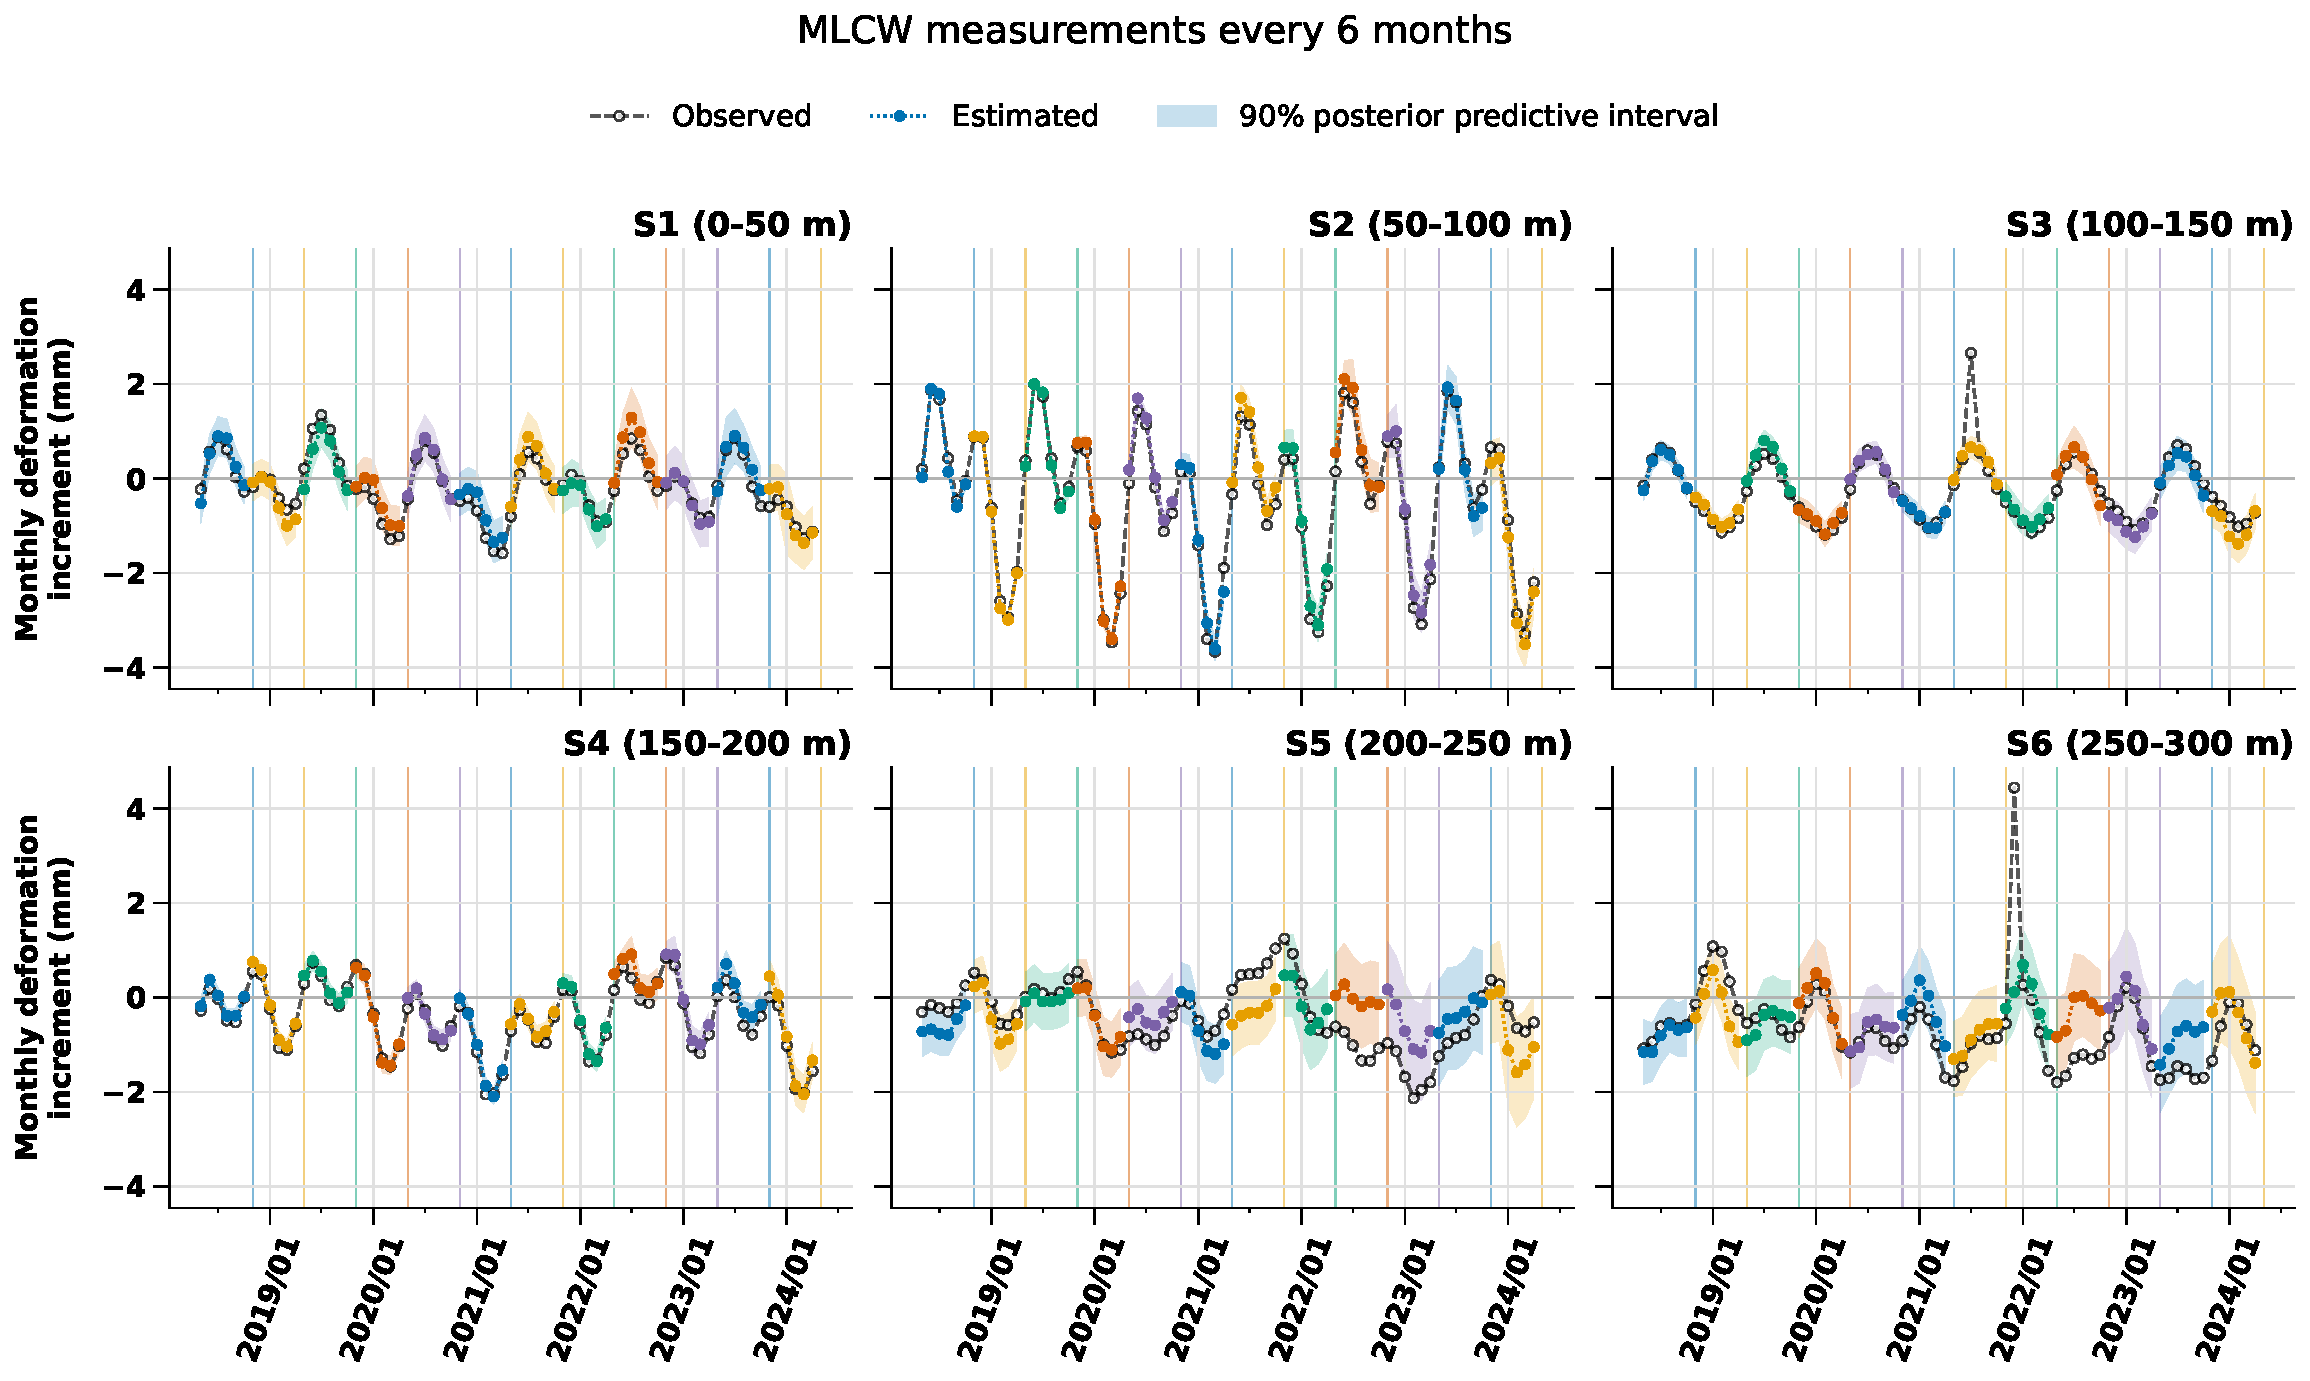
\includegraphics[width=0.98\textwidth]{figures/fig_results_reduced_frequency_3yr_panel_a.pdf}
  \caption[Observed and estimated monthly deformation increments under reduced MLCW measurement frequency.]{Observed and estimated monthly deformation increments for the 3-year initial record, all six depth sections, evaluated over the shared 05/2018--04/2024 period. (a) 6-month measurement schedule. Vertical lines mark the months when a new cumulative MLCW field measurement became available for the next update.}
  \label{fig:results_reduced_frequency_3yr}
\end{figure}

\begin{figure}[tp]
  \ContinuedFloat
  \centering
  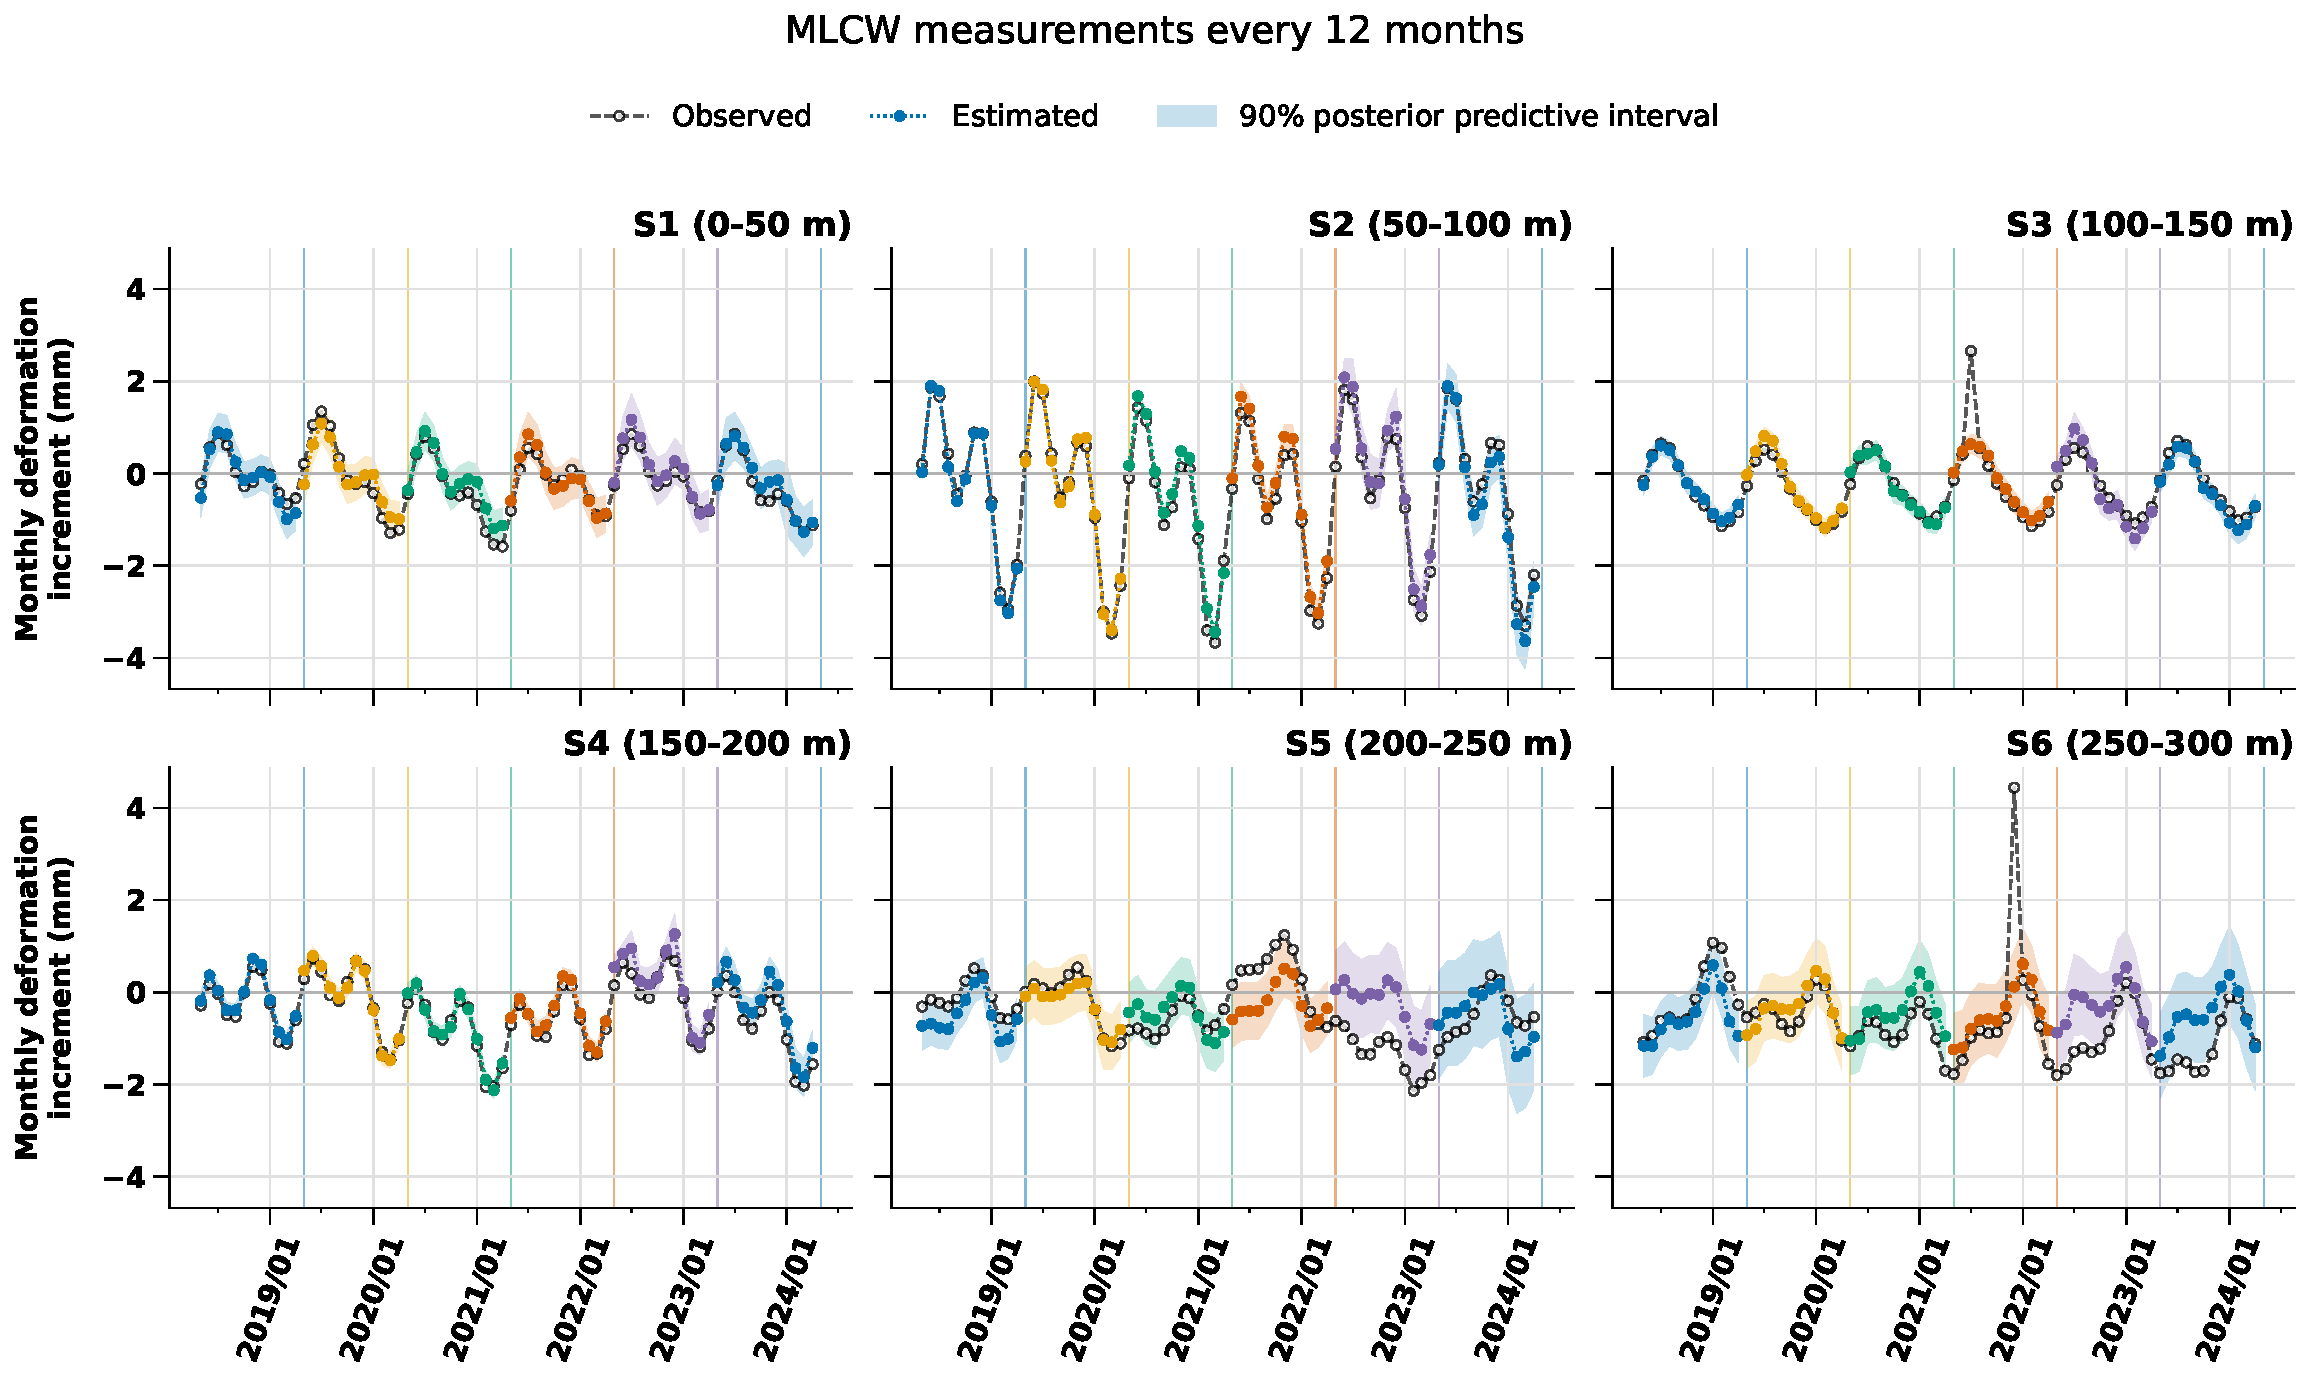
\includegraphics[width=0.98\textwidth]{figures/fig_results_reduced_frequency_3yr_panel_b.pdf}
  \caption[]{(b) 12-month measurement schedule.}
\end{figure}

\FloatBarrier

% Source: diag_28_sec4_meansd_tables.py (sec4_2_meansd.csv; per-section-then-mean+-SD, n=6 sections per row)
\begin{table}[htbp]
  \centering
  \footnotesize
  \setlength{\tabcolsep}{3pt}
  \renewcommand{\arraystretch}{1.2}
  \caption[Monthly errors under reduced MLCW measurement frequency.]{Monthly errors at Tuku, evaluated over the identical 72-month period (05/2018--04/2024) in every scenario. Mean $\pm$ SD, $n=6$ sections; metrics per \Cref{tab:evaluation_metrics}. Full per-section values: \Cref{supp-tab:supp_reduced_frequency_monthly_full}.}
  \label{tab:results_reduced_frequency}
  \begin{tabular}{c|c|r|r|r|r|r}
    \toprule
    \multicolumn{1}{c|}{\shortstack{\textbf{Sampling}\\\textbf{interval}\\\textbf{(months)}}} & \multicolumn{1}{c|}{\shortstack{\textbf{Initial}\\\textbf{record}\\\textbf{(years)}}} & \multicolumn{1}{c|}{\textbf{$R^2$}} & \multicolumn{1}{c|}{\textbf{MAE}} & \multicolumn{1}{c|}{\textbf{RMSE}} & \multicolumn{1}{c|}{\textbf{Coverage (\%)}} & \multicolumn{1}{c}{\textbf{Width}} \\
    \midrule
    6  & 3 & $0.70\pm0.3$ & $0.28\pm0.2$ & $0.37\pm0.2$ & $82.9\pm9.6$ & $0.94\pm0.5$ \\
    6  & 5 & $0.68\pm0.4$ & $0.27\pm0.2$ & $0.38\pm0.3$ & $89.4\pm9.5$ & $1.11\pm0.8$ \\
    6  & 8 & $0.67\pm0.3$ & $0.30\pm0.1$ & $0.40\pm0.2$ & $87.3\pm9.0$ & $1.35\pm0.8$ \\
    \midrule
    12 & 3 & $0.69\pm0.3$ & $0.29\pm0.2$ & $0.39\pm0.2$ & $77.8\pm9.5$ & $0.87\pm0.5$ \\
    12 & 5 & $0.68\pm0.4$ & $0.27\pm0.2$ & $0.38\pm0.2$ & $86.6\pm12.7$ & $1.07\pm0.7$ \\
    12 & 8 & $0.66\pm0.3$ & $0.31\pm0.1$ & $0.41\pm0.2$ & $81.9\pm12.0$ & $1.32\pm0.9$ \\
    \bottomrule
  \end{tabular}
\end{table}

Mean monthly MAE across the six depth sections remained between 0.27 and 0.31~mm/month across the six scenarios (\Cref{tab:results_reduced_frequency}). Mean $R^2$ ranged from 0.66 to 0.70 and did not differ consistently between the 6-month and 12-month schedules. In every scenario the standard deviation across sections was large relative to the mean --- for $R^2$, the standard deviation exceeded 0.3 in all six scenarios --- reflecting the same S1--S4 versus S5--S6 depth contrast already documented in \Cref{subsec:results_delayed_delivery}; full per-section values are given in \Cref{supp-tab:supp_reduced_frequency_monthly_full}.

Extending the initial record from 3 to 8 years did not reduce mean monthly MAE consistently. The 5-year record produced the lowest mean monthly MAE under both schedules, whereas the 8-year record produced the highest. Mean coverage of the nominal 90\% intervals ranged from 77.8 to 89.4\%, remaining below the nominal level in all six scenarios on average. As in \Cref{subsec:results_delayed_delivery}, this shortfall reflects the discrepancy between the observed coverage and the nominal interval level rather than a difference in interval width; possible mechanisms are discussed in \Cref{subsec:discussion_limitations}.

\FloatBarrier

\subsection{Estimation without subsequent MLCW measurements}
\label{subsec:results_no_subsequent_mlcw}

Without subsequent MLCW measurements, monthly errors remained within a narrow range among the three initial-record lengths. Each model was calibrated once and evaluated over the same 80 months from 05/2018 to 12/2024 while monthly hydraulic-head and cGNSS observations remained available. Averaged across the six depth sections, mean monthly MAE ranged from 0.26 to 0.29~mm/month and mean RMSE ranged from 0.36 to 0.40~mm/month across the three initial-record lengths (\Cref{tab:results_no_subsequent_mlcw_interval}).

Cumulative errors varied among depth sections and, by month 80, ended at different values (\Cref{fig:results_no_subsequent_mlcw_cumulative_error}). At the end of the 80-month evaluation period, S4 had the largest absolute cumulative error under all three initial-record lengths (\Cref{tab:results_no_subsequent_mlcw_h80}). The 8-year initial record reduced this error in S4--S6. It did not produce the smallest value in every section. The 5-year record performed better than the 8-year record in S1 and S2.

\begin{figure}[htbp]
  \centering
  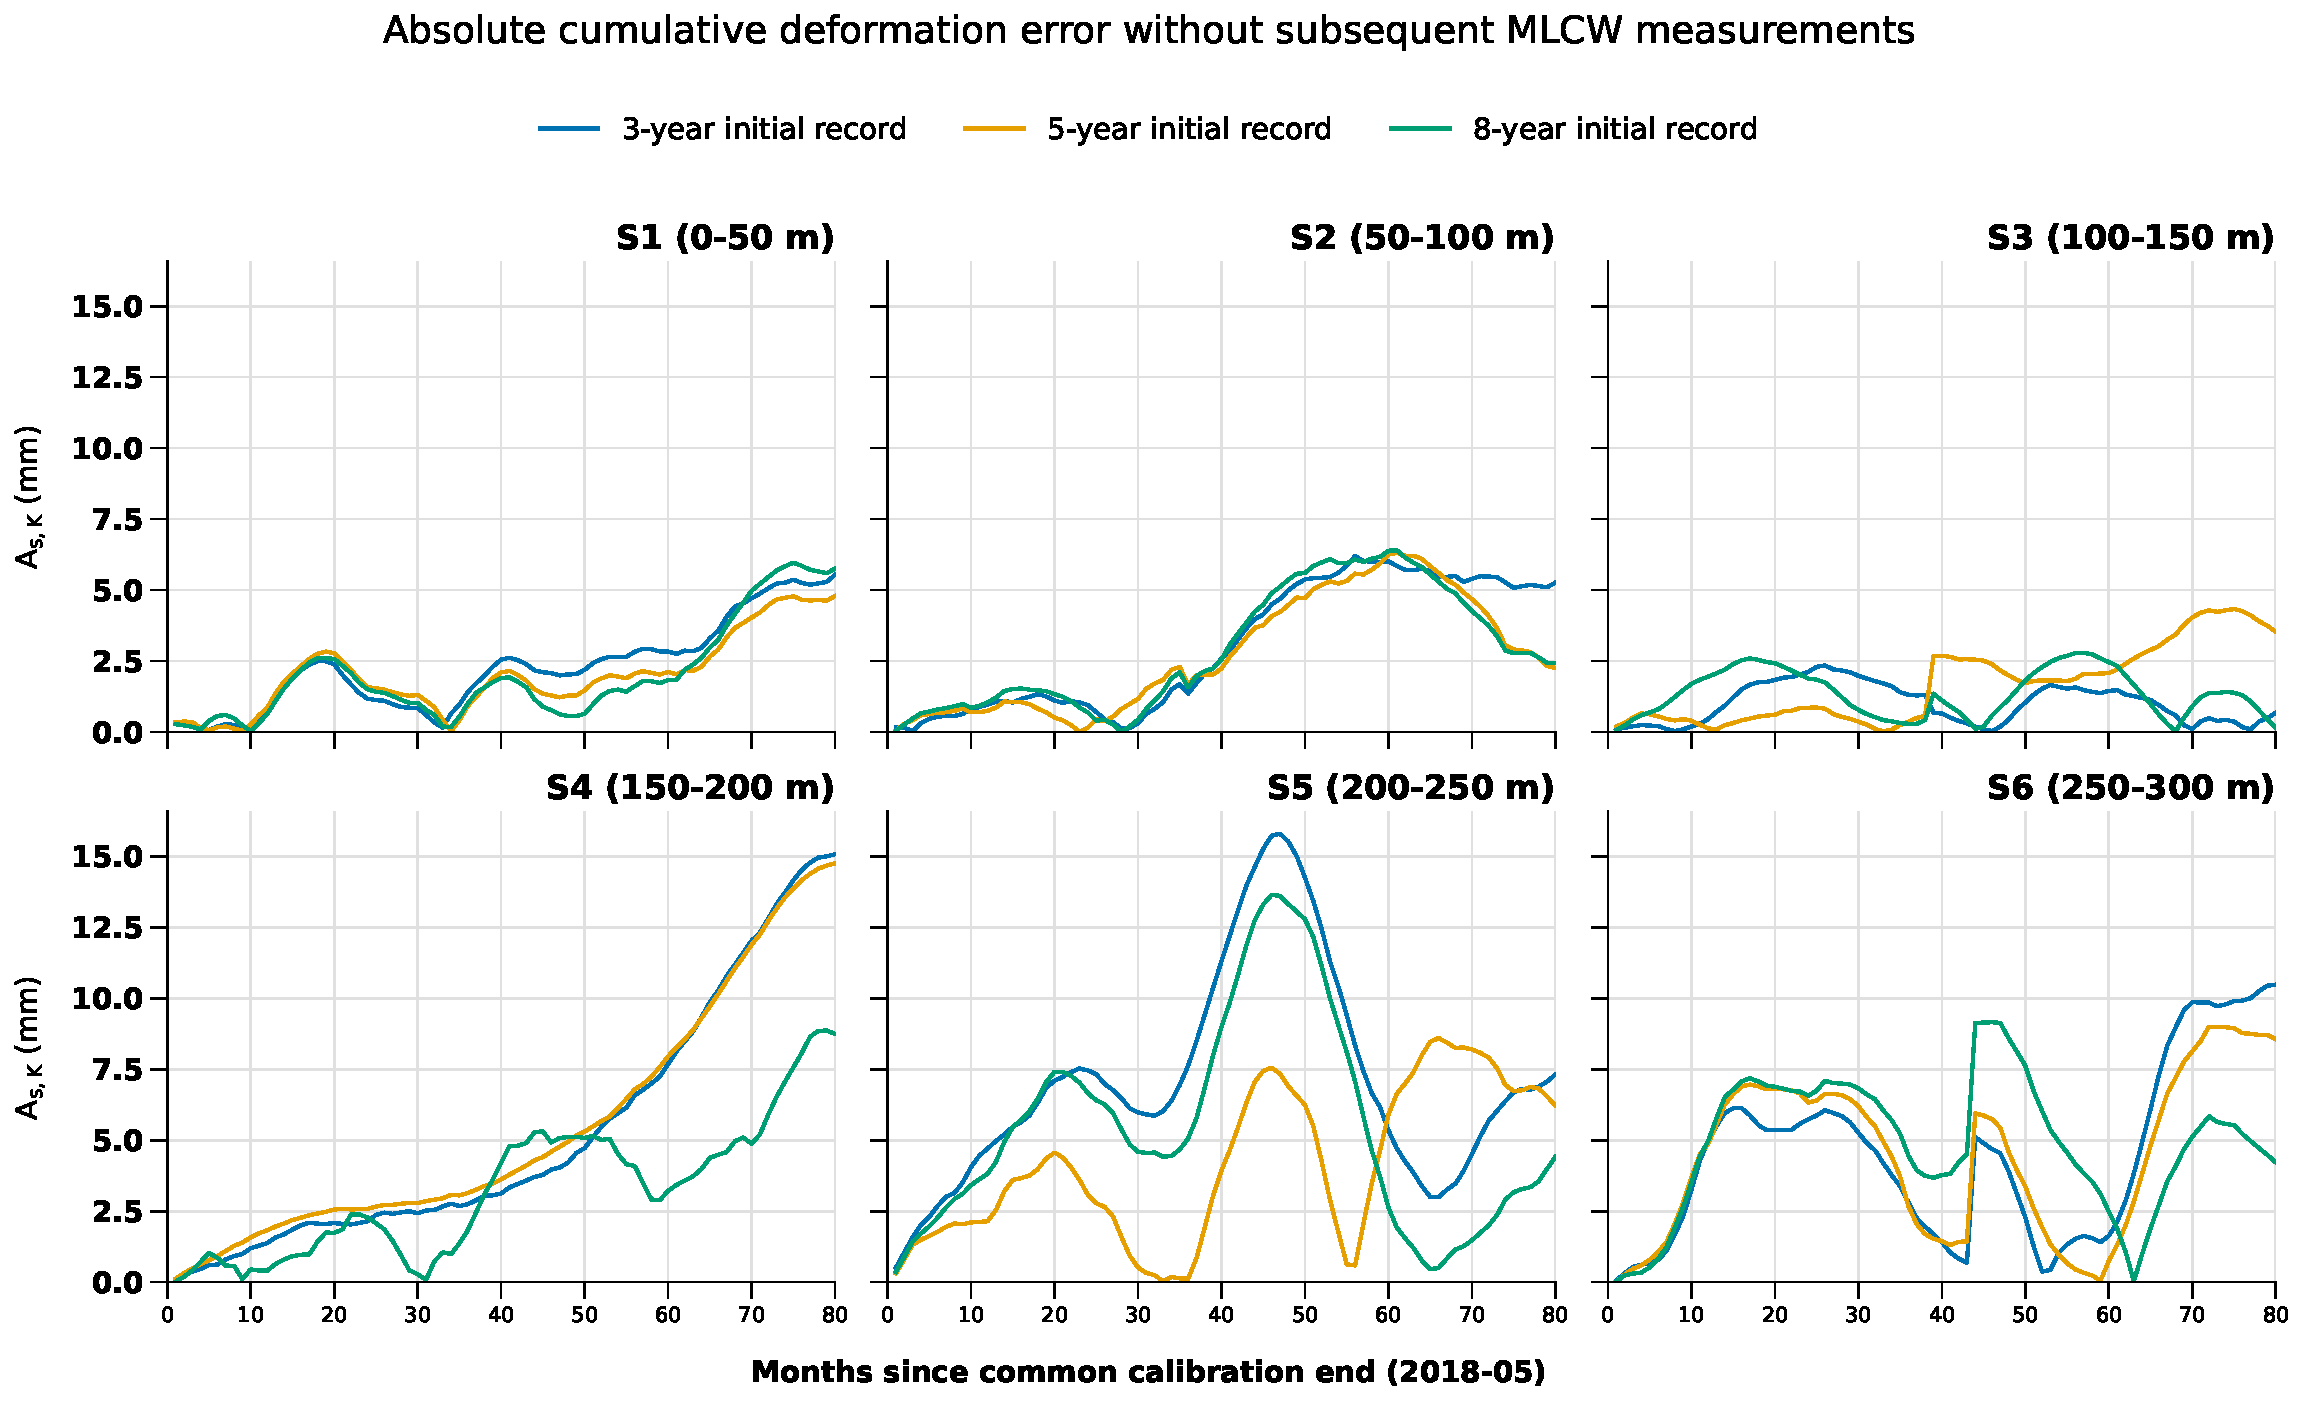
\includegraphics[width=0.98\textwidth]{figures/fig_results_no_subsequent_mlcw_cumulative_error.pdf}
  \caption[Absolute cumulative deformation error without subsequent MLCW measurements.]{Absolute cumulative deformation error $A_{s,K}=|E_{s,K}|$ for each depth section against months since the shared calibration endpoint (05/2018), shown separately for the 3-, 5-, and 8-year initial records, evaluated over the shared 80-month period.}
  \label{fig:results_no_subsequent_mlcw_cumulative_error}
\end{figure}

\begin{table}[htbp]
  \centering
  \small
  \renewcommand{\arraystretch}{1.15}
  \caption[Absolute cumulative deformation error without subsequent MLCW measurements.]{Absolute cumulative deformation error after 80 months without subsequent MLCW measurements. Values give $A_{s,80}=|E_{s,80}|$ in mm for each depth section: the absolute value of the accumulated signed error, not the sum of monthly absolute errors. Models used the stated initial MLCW record, all ending calibration on the same calendar date, and were not updated thereafter. All scenarios span the identical 80-month period (05/2018--12/2024).}
  \label{tab:results_no_subsequent_mlcw_h80}
  \begin{tabular}{l|r|r|r}
    \toprule
    \multicolumn{1}{c|}{\textbf{Section}} & \multicolumn{1}{c|}{\textbf{3-year initial record}} & \multicolumn{1}{c|}{\textbf{5-year initial record}} & \multicolumn{1}{c}{\textbf{8-year initial record}} \\
    \midrule
    S1 & 5.540 & 4.794 & 5.755 \\
    S2 & 5.262 & 2.254 & 2.437 \\
    S3 & 0.687 & 3.530 & 0.139 \\
    S4 & 15.075 & 14.755 & 8.747 \\
    S5 & 7.317 & 6.226 & 4.421 \\
    S6 & 10.480 & 8.555 & 4.217 \\
    \bottomrule
  \end{tabular}
\end{table}

Mean coverage of the nominal 90\% intervals, averaged across the six depth sections, ranged from 65.6 to 79.8\% across the three initial-record lengths, remaining below the nominal level on average in every scenario (\Cref{tab:results_no_subsequent_mlcw_interval}). As in \Cref{subsec:results_delayed_delivery}, this shortfall reflects the discrepancy between the observed coverage and the nominal interval level rather than a difference in interval width; possible mechanisms are discussed in \Cref{subsec:discussion_limitations}.

% Source: diag_28_sec4_meansd_tables.py (sec4_3_meansd.csv; per-section-then-mean+-SD, n=6 sections per row)
\begin{table}[htbp]
  \centering
  \small
  \renewcommand{\arraystretch}{1.2}
  \caption[Monthly error and posterior predictive interval statistics without subsequent MLCW measurements.]{Monthly errors at Tuku, evaluated over the identical 80-month period (05/2018--12/2024) in every scenario. Mean $\pm$ SD, $n=6$ sections; metrics per \Cref{tab:evaluation_metrics}. Full per-section values: \Cref{supp-tab:supp_no_subsequent_mlcw_monthly_full}.}
  \label{tab:results_no_subsequent_mlcw_interval}
  \begin{tabular}{l|r|r|r|r|r}
    \toprule
    \multicolumn{1}{c|}{\shortstack{\textbf{Initial}\\\textbf{record}\\\textbf{(years)}}} & \multicolumn{1}{c|}{\textbf{$R^2$}} & \multicolumn{1}{c|}{\textbf{MAE}} & \multicolumn{1}{c|}{\textbf{RMSE}} & \multicolumn{1}{c|}{\textbf{Coverage (\%)}} & \multicolumn{1}{c}{\textbf{Width}} \\
    \midrule
    3 & $0.71\pm0.3$ & $0.26\pm0.1$ & $0.36\pm0.2$ & $65.6\pm18.4$ & $0.62\pm0.3$ \\
    5 & $0.70\pm0.3$ & $0.26\pm0.1$ & $0.37\pm0.2$ & $79.8\pm26.0$ & $0.97\pm0.7$ \\
    8 & $0.67\pm0.3$ & $0.29\pm0.1$ & $0.40\pm0.2$ & $78.8\pm19.1$ & $1.23\pm0.9$ \\
    \bottomrule
  \end{tabular}
\end{table}

\FloatBarrier


\section{Discussion}
\label{sec:discussion}
% Discussion draft. The detailed interpretation will be written after the
% Results section has been completed and reviewed.

Hydraulic head, vertical surface displacement, and seasonal observations supported monthly layerwise deformation estimation at Tuku under all three conditions of MLCW information. The evidence was strongest in S1--S4 and less uniform in S5--S6. Reduced MLCW information was not accompanied by the same immediate change in monthly error in every tested case, but it reduced the frequency of independent depth-specific checks on accumulated deformation.
% NOTE: Đoạn mở đầu trả lời ba ý chính: các quan trắc hỗ trợ ước lượng hằng tháng, bằng chứng thay đổi theo độ sâu, và ít thông tin MLCW hơn đồng nghĩa với ít lần kiểm tra tích lũy độc lập theo độ sâu hơn. %

\subsection{Layerwise monthly deformation estimation}
\label{subsec:discussion_layerwise_estimation}

Monthly deformation estimation depended on how the continuous observations represented conditions within each depth section. The cGNSS record represents the integrated surface response, whereas MLCW observations separate deformation among monitored depth intervals \citep{hung_measuring_2021}. A station-scale displacement signal can therefore contribute to monthly estimation without representing every section equally well. This distinction makes the contrast between S1--S4 and S5--S6 central to evaluating the depth information recovered from the continuous records.

Monthly estimates in S1--S4 had $R^2$ values from 0.80 to 0.98. Their MAE values ranged from 0.15 to 0.26~mm/month. In S5 and S6, $R^2$ was 0.08 and 0.34 and MAE was 0.50 and 0.40~mm/month, respectively. RMSE showed the same depth division, reaching 0.66 and 0.62~mm/month in S5 and S6 compared with 0.21--0.31~mm/month in S1--S4. These point metrics establish the depth contrast but do not distinguish differences in variability from differences in the temporal pattern.
% my note : tui nghĩ chúng ta có thể sử dụng respectively để nói về các elevaluation metrics của S5 và S6, bởi vì chỉ có 2 giá trị thôi, không cần dùng cấu trúc 'from ... to ...' %
% my note : corresponding ranges này là sao? là so sánh giữa 1 nhóm từ S1 tới S4, với nhóm từ S5 tới S6 hả? nếu đúng là như vậy thì cách viết này làm tui không hiểu ngay khi lần đầu đọc qua. với một người làm việc xuyên suốt với dự án mà còn không hiểu thì làm sao một độc giả xa lạ sẽ hiểu được??? %
% my note : bạn viết đoạn này là có ý gì, tui chưa hiểu lắm, tui không hiểu bạn muốn truyền tải điều gì ở đây, nó có kết nối gì với phần results, và nó sẽ mở ra điều gì cho các phần thảo luận bên dưới? %

The supplementary diagnostics separate these two aspects of the estimates (\Cref{app:variability_diagnostics,supp-tab:supp_delayed_variability_diagnostics}). In S1--S4, estimated-to-observed standard-deviation ratios of 0.89--0.98 were accompanied by temporal correlations of 0.93--0.99, showing that the estimates reproduced both the observed variability and its temporal pattern. The corresponding ratios and correlations decreased to 0.50 and 0.35 in S5 and 0.65 and 0.59 in S6. The lower performance in S5--S6 was therefore associated with both damped variability and lower temporal agreement, rather than average error alone.

This depth dependence is consistent with the information available to the separately fitted section models. Each model combined the same integrated surface-displacement record with hydraulic-head and seasonal variables that represented conditions for its target section. The current surface-displacement coefficient remained positive across model updates in S1--S4 and S6, whereas its 10th--90th percentile range crossed zero in S5, indicating that its fitted direction varied among updates (\Cref{tab:selected_coefficients}). The current, lagged, and trailing-average predictors also contained overlapping temporal information, so Bayesian ridge regression distributed their shared information across coefficients and limited changes in relations with less observational support \citep{dormann_collinearity_2013, hastie_elements_2009, mackay_bayesian_1992}. Hydraulic-head representation supplied depth-specific information to the models, while sediment composition provided context for interpreting differences among sections. The coefficient patterns establish that the fitted observational relations differed across the monitored profile.
% NOTE: Đoạn này giải thích hành vi của mô hình và sự khác nhau giữa các section, nhưng không diễn giải coefficient như bằng chứng nhân quả. %
% my note: tui không thấy các câu hỏi mà tui đặt ra ở results004.tex được thảo luận ở đây. cho dù ta có phải chạy thêm phân tích, tìm thêm trích dẫn, ta phải tìm cách để thảo luận 'tại sao kết quả lại như vậy? về mặt toán học, tại sao? về mặt vật lý, có thể là do những lý do nào?' %

Depth dependence also appeared in the posterior predictive intervals. Empirical coverage below 90\% means that the intervals enclosed fewer observations than their nominal level implies. S5 had a mean interval width of 1.85~mm/month and coverage of 81.2\%, whereas S6 had a narrower interval of 0.97~mm/month and lower coverage of 65.9\%. A wider interval encloses a larger range of plausible values and can therefore contain more observations even when its point estimates have larger errors. Higher coverage in S5 consequently did not indicate smaller point errors, making coverage and interval width necessary companion measures \citep{gneiting_probabilistic_2007, gelman_bayesian_2013}.
% NOTE: Khoảng rộng hơn có thể bao phủ nhiều quan trắc hơn nhưng kém chính xác hơn; vì vậy coverage và width phải được đọc cùng nhau, không dùng riêng coverage để kết luận S5 được ước lượng tốt hơn S6. %

Evaluation by month position addressed whether estimation performance deteriorated as each delayed-delivery cycle progressed. The errors did not increase steadily because each monthly increment was estimated from hydraulic-head and surface-displacement observations for that month, without using a previously estimated MLCW increment as a predictor. An error in one month was therefore not passed to the next month as a model input. Each estimate remained tied to its own contemporaneous observations rather than to an accumulating chain of earlier estimates.
% NOTE: Kết quả không cho thấy sai số tăng đều theo vị trí tháng trong chu kỳ giao MLCW trễ vì mỗi ước lượng tháng dùng quan trắc hydraulic head và chuyển dịch bề mặt cùng tháng, không dùng ước lượng MLCW của tháng trước làm biến đầu vào. Sai số của một tháng vì vậy không được truyền đệ quy sang tháng sau, nhưng thiết kế này không giải thích cơ chế vật lý hay bảo đảm hiệu năng cho các tháng sau. %

At the same TKJS monitoring site, \citet{hung2025_realtime} showed that high-frequency extensometers and MLCWs provide complementary temporal and depth resolution. The present study addressed a different monitoring need by estimating monthly deformation within individual depth sections from continuous hydraulic-head and surface-displacement observations between MLCW updates. Periodic access to finalized MLCW observations provided the direct measurements needed to resolve and evaluate deformation across the monitored profile. Together, these results show that continuous observations can support monthly depth-section estimation between MLCW updates, while MLCW records provide the direct depth-specific calibration and evaluation needed across the monitored profile.

\subsection{Estimation with reduced MLCW information}
\label{subsec:discussion_reduced_mlcw_information}

The effect of reducing MLCW information was not uniform across the tested measurement scenarios. The paired comparison used a matched 72-month observation window, with the same dataset, the same 38 predictors, and the same section-month observations for reduced-frequency and delayed monthly-record estimation. Four of the six 95\% resampling intervals for the MAE difference included zero and therefore did not establish a stable direction of change, whereas the two cases based on the 8-year initial record had higher MAE than the delayed monthly-record reference. An interval that contains zero is inconclusive about the direction of the difference and does not establish equivalent performance, as defined in \Cref{app:paired_mae_comparisons}. Reduced measurement frequency therefore produced no single monthly-error response across the tested cases at Tuku.
% NOTE: So sánh trên cùng cửa sổ 72 tháng, cùng bộ dữ liệu, 38 biến dự báo và các quan trắc section-tháng cho thấy bốn trường hợp chưa xác định được hướng thay đổi ổn định; điều này hẹp hơn kết luận không có ảnh hưởng hoặc tương đương. %

This heterogeneity also appeared when the initial record increased from 3 to 5 to 8 years. Monthly MAE did not decline monotonically under either measurement schedule, and the 8-year record had higher MAE than the 5-year record under both schedules. One interpretation is that a longer initial record adds observations from an earlier and different calendar period, whose fitted relations may not represent the later evaluation period more closely. This explanation was not tested as a mechanism. The evidence therefore rejects the assumption that more history always improves estimation, but it does not identify a minimum or preferred initial-record length.
% NOTE: Việc thêm các năm sớm hơn có thể giải thích pattern nhưng chưa được kiểm định như một mechanism; kết quả chỉ bác bỏ giả định rằng lịch sử dài hơn luôn tốt hơn, không chọn độ dài chuỗi ban đầu. %

Monthly and endpoint errors separate the performance of individual estimates from the discrepancy accumulated between field measurements. Average monthly MAE occupied a narrow range across the six reduced-frequency scenarios. The 12-month endpoints aggregated twice as many monthly estimates as the 6-month endpoints, and endpoint MAE was higher in the tested scenarios. Signed errors can add to or offset one another across those monthly estimates. This endpoint comparison does not show whether the cumulative discrepancy over any six-month portion of a 12-month schedule was smaller or larger than the endpoint discrepancy for a complete six-month schedule. Each new MLCW measurement both updates the fitted model and provides an independent depth-specific check on cumulative deformation, so the endpoint discrepancy reflects the duration between those checks as well as the monthly errors.
% NOTE: Sai số hằng tháng mô tả từng ước lượng, còn sai lệch tại endpoint tích lũy qua toàn khoảng đo; số liệu hiện có không so sánh riêng sáu tháng đầu của lịch 12 tháng với một lịch 6 tháng hoàn chỉnh. %

The absence of the next MLCW checkpoint extends this accumulation beyond the reduced-frequency design. Monthly MAE remained similar among the 3-, 5-, and 8-year initial records, while signed monthly errors added to or offset earlier errors and changed the ordering of cumulative-error trajectories over time and among depth sections. The 8-year record had the lowest average absolute cumulative error at month 80, but not throughout the evaluation period or in every section. Monthly agreement and cumulative agreement therefore answer different questions, and the final ordering does not identify a preferred initial record or support ending MLCW measurements.
% NOTE: Sai số hằng tháng gần nhau không bảo đảm sai lệch tích lũy gần nhau; thứ tự tại tháng 80 không đại diện cho toàn bộ thời gian hoặc mọi section. %

Under the tested Tuku conditions, reduced MLCW information was not accompanied by an immediate and uniform loss of monthly performance. Fewer MLCW measurements nevertheless provided fewer independent opportunities to check accumulated depth-specific deformation. This distinction is a scientific implication of the tested scenarios rather than a field schedule, and its practical interpretation must remain within the evidence boundary established at Tuku.
% NOTE: Đây là hàm ý khoa học về vai trò kiểm tra tích lũy của MLCW, không phải một lịch đo thực địa được đề xuất. %

\subsection{Limitations and practical scope}
\label{subsec:discussion_limitations}

The evidence establishes performance for the tested monitoring record at Tuku. The contrast between S1--S4 and S5--S6 shows that estimation performance varied among depth sections even within this single site, without identifying a physical cause for that pattern. The results therefore do not establish the same performance at other monitoring stations or in every depth interval. Tuku instead provides a detailed evaluation of the framework within one instrumented monitoring system.
% NOTE: Bằng chứng tại Tuku có giá trị như một đánh giá chi tiết tại một trạm, nhưng sự khác nhau giữa các section cho thấy không thể mặc định cùng mức performance ở mọi trạm hoặc mọi khoảng độ sâu. %

The Bayesian ridge coefficients describe fitted associations within the Tuku calibration record, not physical mechanisms. The regression does not replace a coupled groundwater-flow and aquifer-system-deformation model. The supporting records differ in observational scope. cGNSS represents vertical deformation integrated over the underlying aquifer system, including deformation below the approximately 300~m MLCW monitored depth; hydraulic head represents measured or interpolated groundwater conditions; and lithology provides context for interpreting the depth sections but was not a model input. Consequently, coefficient signs and magnitudes do not prove that a particular hydraulic-head or surface-displacement variable causes deformation in a section.
% NOTE: Đoạn này tách fitted associations khỏi cơ chế vật lý và làm rõ phạm vi quan trắc của cGNSS, hydraulic head và lithology; lithology chỉ hỗ trợ diễn giải chứ không đi vào mô hình. %

The posterior predictive intervals include coefficient uncertainty and residual variation represented by the fitted model \citep{gelman_bayesian_2013, gneiting_probabilistic_2007}. They do not automatically include every source of uncertainty associated with field measurements, temporal alignment, interpolated hydraulic head, model form, or dependence among residuals. These omitted sources are plausible contributors to empirical coverage below the nominal level, but the current evaluation does not demonstrate that any one of them caused the undercoverage. The intervals are model-based, whereas empirical coverage is the observed frequency with which those intervals contained observations; together, they do not provide complete descriptions of observational uncertainty.
% NOTE: Khoảng dự báo phản ánh uncertainty mà mô hình biểu diễn, không phải toàn bộ uncertainty ngoài thực địa; các nguồn bị bỏ sót chỉ là khả năng góp phần vào undercoverage, chưa phải nguyên nhân đã được chứng minh. %

Within these boundaries, the framework quantifies monthly estimation error, cumulative discrepancy, and model-based uncertainty under three levels of MLCW information at Tuku. These quantities make the monitoring consequences of reduced MLCW information explicit without defining an acceptable operational error threshold, an economic decision rule, or a measurement schedule suitable for all settings. The bounded contribution is a common evidence base for evaluating monthly and accumulated estimation performance as MLCW information decreases at a well-instrumented site.
% NOTE: Đóng góp chính là định lượng rõ sai số hằng tháng, sai lệch tích lũy và uncertainty theo mô hình để đánh giá hệ quả khi thông tin MLCW giảm, không phải đưa ra một lịch đo áp dụng cho mọi nơi. %

\FloatBarrier


\section{Conclusions}
\label{sec:conclusions}
The objective of this study was to estimate monthly depth-resolved compaction at the Tuku monitoring site during a six-month period in which finalised MLCW measurements were temporarily unavailable. One independent Bayesian ridge regression model was developed for each of six standardised 50~m depth sections using contemporaneous hydraulic head changes, vertical surface displacement increments, sediment composition, and seasonal terms as predictors.

The walk-forward evaluation showed that monthly compaction estimates reproduced the observed section-level MLCW increments with $R^2$ values ranging from \placeholder{MIN R2} to \placeholder{MAX R2} in sections S1 through S4. Performance was weaker in the two deepest sections, where the available piezometric observations did not screen the principal compacting deposits. Bayesian predictive intervals attained empirical coverage of \placeholder{COVERAGE RANGE} across the evaluated sections, providing calibrated uncertainty bounds for each monthly estimate from the first evaluation block onward. Under hypothetical reduced-frequency measurement schedules, the model distributed compaction among unobserved months with a monthly MAE of \placeholder{BEST H6 MAE} to \placeholder{WORST H6 MAE}~mm/month at the six-month interval, while cumulative endpoint errors remained within \placeholder{ENDPOINT RANGE}~mm of the observed field measurements.

These results demonstrated that contemporaneous hydraulic and surface displacement records can bridge a known data delay and provide provisional monthly estimates of section-level compaction at a single well-instrumented site. The model preserved direct MLCW observations as the reference measurement, using them to evaluate, constrain, and update the estimates when the finalised records became available. Extension to additional MLCW stations is required before the approach can support broader monitoring applications across the Choushui River Alluvial Fan.

\FloatBarrier


%\section*{Acknowledgements}
%\placeholder{FUNDING, DATA PROVIDERS, AND CONTRIBUTOR ACKNOWLEDGEMENTS}
%
%\section*{Author contributions}
%\placeholder{AUTHOR CONTRIBUTION STATEMENT}
%
%\section*{Data availability}
%\placeholder{DATA AND CODE AVAILABILITY STATEMENT}
%
%\section*{Conflict of interest}
%\placeholder{CONFLICT OF INTEREST STATEMENT}

\clearpage
\appendix
\section{Supplementary methodological details}
\label{app:methods}

\subsection{Final predictor inventory}
\label{app:predictors}

Each section model used 38 predictor variables, grouped below by the physical information they represent. Vertical surface displacement was represented by the current cGNSS increment, its second difference, and its one- and three-month lags. Hydraulic head was represented by the current head change, its second difference, its one-, three-, six-, twelve-, and twenty-four-month lags, three- and six-month rolling means of head change, and the absolute value of head change. Seasonal variation was represented by annual and semiannual sine and cosine terms, a dry-season indicator, and the interaction of head change with the dry-season indicator. Cross-section hydraulic conditions were represented by the current head change and its three- and six-month rolling means, computed separately for each of the six depth sections. Every predictor was available for the target month at the time each estimate was produced. The exact variable names, source columns, and lag definitions used to reproduce the analysis are recorded in the analysis repository's frozen feature manifest (internal identifier \texttt{feature\_manifest.json}, run \texttt{run\_048}); that manifest is the reproducibility record and is not reproduced verbatim here.

\subsection{Model fitting and update settings}
\label{app:model_settings}

The reproducibility record will report the initial calibration period, the six-month block boundaries, the predictor scaling procedure, the fitted regression settings, and the rules used when an input observation was unavailable. \placeholder{INSERT VERIFIED MODEL SETTINGS AND SOFTWARE ENVIRONMENT FROM THE FINAL RUN}. These details will reproduce the reported estimates without interrupting the main methodological narrative.

\subsection{Prediction interval calibration}
\label{app:intervals}

Because the independent section models were fitted using Bayesian ridge regression, the prediction intervals were derived analytically from the posterior predictive distribution. Unlike empirical quantile methods that require an accumulated error archive, the Bayesian formulation provided a theoretically justified interval for every point estimate beginning with the first evaluation block. The prior distribution and noise precision parameters were estimated directly from the available calibration data during each model update. The resulting posterior covariance matrix of the coefficients, combined with the estimated noise precision, defined the uncertainty for each subsequent prediction.

\subsection{Reduced-frequency MLCW measurement settings}
\label{app:sparse_measurement_settings}
\label{app:no_update_settings}

The reduced-frequency analysis contained six scenarios defined by measurement intervals of six or twelve months and initial calibration periods of 36, 60, or 96 consecutive months. The three calibration periods shared a common endpoint rather than a common start, so the 36- and 60-month periods began later than the 96-month period. Each scenario's subsequent evaluation continued through a shared field-measurement endpoint common to both measurement schedules, so the three initial-history lengths within one schedule underwent the same number of model updates at the same calendar dates; the six-month and twelve-month schedules were not required to share the same update count with each other, since sampling frequency was itself the quantity under comparison. Incomplete intervals at the end of the shared evaluation period were excluded.

For depth section $s$ and measurement interval $I$, the endpoint observation was the accumulated MLCW deformation,
\begin{equation}
\Delta d_{s,I}
=
\sum_{k\in I}\Delta d_{s,k},
\label{eq:interval_compaction}
\end{equation}
where $k$ denotes a monthly epoch and $\Delta d_{s,k}$ denotes the observed monthly deformation increment retained for retrospective evaluation. The endpoint observation constrained the update before the next interval, whereas the individual values of $\Delta d_{s,k}$ within $I$ remained unavailable to the model. \placeholder{INSERT THE VERIFIED NUMERICAL FORMULATION AND WEIGHTING OF THE ENDPOINT CONSTRAINT FROM THE FROZEN IMPLEMENTATION}.

The monthly error was

\begin{equation}
e_{s,k}
=
\widehat{\Delta d}_{s,k}
-
\Delta d_{s,k}.
\label{eq:appendix_monthly_error}
\end{equation}

The endpoint error was defined as accumulated estimated deformation minus accumulated observed deformation,
\begin{equation}
e_{s,I}
=
\sum_{k\in I}\widehat{\Delta d}_{s,k}
-
\Delta d_{s,I}.
\label{eq:endpoint_error}
\end{equation}
Positive errors represented estimates that were more positive than the observed values. Monthly and endpoint MAE, RMSE, and mean signed error were reported by measurement interval, initial calibration period, and depth section, with pooled values calculated across all six sections. Endpoint totals were not evaluated with the coefficient of determination. The monthly prediction intervals described in \Cref{subsec:predictive_uncertainty} were calculated for the delayed-data analysis, the reduced-frequency analysis, and the analysis without subsequent MLCW measurements. Each interval came from the Bayesian ridge model fitted for that specific scenario; intervals were never combined across scenarios or across measurement schedules.

\FloatBarrier


\bibliography{writing_manu2}

\end{document}
